\documentclass[11pt]{article}

\usepackage[a4paper,margin=1in]{geometry}
\usepackage{amsmath,amssymb,amsthm,mathtools}
\usepackage{booktabs}
\usepackage{array}
\usepackage{tabularx}
\usepackage{enumitem}
\usepackage{bm}
\usepackage{microtype}
\usepackage{hyperref}
\usepackage{xcolor}
\usepackage{graphicx}
\graphicspath{{../figures/}}
\setlength{\emergencystretch}{1.5em}

\hypersetup{
  colorlinks=true,
  linkcolor=blue!60!black,
  citecolor=blue!60!black,
  urlcolor=blue!60!black
}

\newtheorem{theorem}{Theorem}[section]
\newtheorem{proposition}[theorem]{Proposition}
\newtheorem{lemma}[theorem]{Lemma}
\newtheorem{corollary}[theorem]{Corollary}
\theoremstyle{definition}
\newtheorem{assumption}{Assumption}[section]
\newtheorem{definition}[theorem]{Definition}
\newtheorem{remark}[theorem]{Remark}

\newcommand{\indep}{\perp\!\!\!\perp}
\newcommand{\E}{\mathbb{E}}
\newcommand{\Pp}{\mathbb{P}}
\newcommand{\Var}{\operatorname{Var}}
\newcommand{\Cov}{\operatorname{Cov}}
\newcommand{\op}{o_{\mathbb{P}}}
\newcommand{\Op}{O_{\mathbb{P}}}
\newcommand{\R}{\mathbb{R}}
\newcommand{\calT}{\mathcal{T}}
\newcommand{\calI}{\mathcal{I}}
\newcommand{\bfZ}{\mathbf{Z}}
\newcommand{\bfeps}{\boldsymbol{\varepsilon}}
\newcommand{\bfxi}{\boldsymbol{\xi}}
\newcommand{\bfDelta}{\boldsymbol{\Delta}}

\title{Conditional Independence Testing beyond i.i.d. Data:\\
A Taxonomy and Residual-Score Framework}
\author{Qingzi Huo, Marco Simnacher, Xiaotian Xu, and Sonja Greven\\
for the Alzheimer's Disease Neuroimaging Initiative}
\date{Working manuscript, 24 August 2026}

\begin{document}
\maketitle

\begin{abstract}
Conditional-independence testing (CIT) with non-i.i.d. data is not one problem: the valid
conditioning information, the independent sampling unit, and the object being tested all
change across applications. We organise these differences into five cases. Case A concerns
state-level hypotheses $X_{it}\indep Y_{it}\mid Z_{it}$ under three asymptotic regimes: many
short clusters, one or a few long sequences, and double asymptotics. Case B adds stable
subject information $\theta_i$; Case C adds observed history $H_{it}$; Cases D and E
concern conditional independence between entire trajectories, without and with subject
information. This taxonomy separates hypotheses that only require an enlarged conditioning
set from those that require latent-variable identification or genuinely temporal inference.

We then develop a residual-score framework for Cases A--C. In the theoretically developed
many-subject regime, nuisance regressions are cross-fitted by subject, visit-level residual
products are aggregated into one score per subject, and inference is based on the
$\sqrt N$ distribution of independent subject scores. Generalised additive mixed models are
one nuisance learner, not a defining component: other regressions or pre-trained embeddings
may be used when their prediction errors satisfy the stated product-rate and cross-term
conditions. Observed subject information in Case B can be added to the conditioning set;
latent or estimated subject information requires separate identification and rate
conditions. Case C has two internal regimes: a fixed bounded history with many subjects
(C1), which can be included as observed context, and a growing filtration or one/few long
series (C2), which requires temporal weak-dependence or martingale theory outside the present
cluster theorem.

Simulation evidence reflects these boundaries. The core Case-A null yielded 47 rejections
in 1,000 repetitions, but a random-slope stress setting failed the pre-specified calibration
gate. New Case-B and Case-C1 simulations distinguish valid observed-context analyses from
sparse latent-context estimation and incomplete-history reductions. A supplementary gradient
shows how Case-B calibration depends on the accuracy of an independently estimated subject
context and provides local-power curves for observed Case B and complete-history C1. In ADNI
applications, MRI, plasma biomarkers, amyloid PET, cognition, genetics, and acquisition
variables instantiate Case A with many participants and sparse visits. The analyses show how
incremental-information conclusions change with the reference set and identify p-tau217 and
A$\beta$42/40 as plasma markers retaining information about PET amyloid beyond cognition,
demographics, APOE, and acquisition context. A prospective observed-history analysis further
identified p-tau217 as the only plasma marker retaining unique information about future
ADAS-Cog13. Repeating the subject-fold assignment preserved the plasma--amyloid marker
distinction in all 20 assignments and the prospective p-tau217 direction in all 20, although
one prospective split crossed the multiplicity-adjusted 0.05 threshold. Cases D and E, and
single-series temporal inference, remain future work.
\end{abstract}

\newpage
\tableofcontents
\newpage

% ============================================================
\section{Introduction}

Many biomedical, behavioural, and sensor studies ask an incremental-information question:
does a candidate measurement tell us something about an outcome after the information already
available from clinical, behavioural, demographic, or technical variables has been taken into
account? Conditional-independence testing gives this question a direct statistical form. The
generalised covariance measure (GCM) estimates two conditional means and tests whether the
product of their residuals has expectation zero \cite{shahpeters}. Its flexibility comes from
allowing a broad class of regression methods, but its standard theory is formulated for
independent observations.

The phrase ``non-i.i.d. CIT'' hides several distinct problems. Repeated measurements from
many subjects create independent clusters; one long time series instead has no replication
across subjects; stable subject information may be observed, estimated, or latent; and a null
about current measurements is not the same as a null about complete trajectories. These
distinctions determine what must enter the conditioning set, what is asymptotically
independent, and which central limit theorem can justify a reference distribution. Treating
all of them as a generic mixed-model correction changes the hypothesis without resolving the
sampling problem.

We begin with a five-case taxonomy organised by the object of inference and the
available information. It then develops a common residual-score construction for the cases
that can be reduced to conditional-mean estimation plus an appropriate score-level central
limit theorem. For many independent subjects, visit-level residual products are aggregated
into one score per subject. Nuisance models are cross-fitted by subject, predictions for held-
out subjects exclude subject-specific BLUPs in a population analysis, and inference uses the
empirical variance of complete subject scores. A Gaussian multiplier extends the construction
to several candidate markers.

The three contributions are:
\begin{enumerate}[leftmargin=*]
\item \textbf{A problem map for non-i.i.d. CIT.} We distinguish five nulls (Cases A--E),
three asymptotic regimes inside Case A, and observed versus latent subject information inside
Case B. The map makes the required domain knowledge and the unsolved identification problems
explicit.
\item \textbf{A residual-score framework with an explicit scope.} We develop the cluster
construction and high-level rate conditions for Case A1. Case B with observed subject
information and Case C1 with complete bounded history can be reduced to Case A1 by enlarging
the conditioning set. Estimated or latent subject information, growing-history Case C2, and
double asymptotics require additional assumptions and are presented separately.
The nuisance learner may be a GAMM, random forest, kernel method, neural network, or a
pre-trained embedding, provided the relevant prediction and leakage conditions hold.
\item \textbf{Evidence across the map.} Existing simulations evaluate Case A and expose a
random-slope limitation and a failed sparse-BLUP construction. New simulations isolate the
roles of observed or estimated subject context and complete or incomplete history, quantify
the proxy-accuracy gradient for generated subject context, and supply local-power curves. ADNI
analyses instantiate the many-subject, sparse-visit regime and evaluate whether imaging and
plasma measurements add information beyond explicitly named clinical, historical, and genetic
reference sets. A prospective application links this question to future cognitive status,
and repeated subject-fold analyses assess dependence on one cross-fitting split.
\end{enumerate}

Two boundaries are maintained throughout. First, the scalar residual score targets an
expected conditional covariance: conditional independence implies a zero target, but the
converse need not hold. Second, incremental information is not a causal effect. Rich
transformations, multivariate scores, or embedding-based CITs can broaden the detected
alternative class, but they do not remove the need to match the null, conditioning set, and
sampling regime.

% ============================================================
\section{A taxonomy of conditional-independence problems beyond i.i.d. data}

Let $i$ index subjects or clusters and $t$ index occasions. Write
$\bar X_{it}=(X_{i1},\ldots,X_{it})$, with analogous notation for $\bar Y_{it}$ and
$\bar Z_{it}$. Let $H_{it}$ denote pre-specified observed history available before the tested
response, and let
$\theta_i$ denote stable subject information. The five cases differ in the random object
being tested and in whether the additional context is observed.

For i.i.d. observations, the literature can be grouped by what is learned under the null.
Kernel and operator methods encode conditional association in reproducing-kernel Hilbert
spaces \cite{fukumizu2007,zhang2011}; residual and prediction methods compare conditional
means or risks, including GCM and its weighted extension \cite{shahpeters,scheidegger2022};
and model-X or generative methods approximate a conditional distribution
\cite{bellot2019}. The GCM deliberately trades omnibus power for transparent regression-rate
requirements. Non-i.i.d. extensions must add a second layer: a valid approximation for the
dependent score process. This is not a cosmetic variance correction. For example, an
i.i.d. bootstrap for kernel independence can fail for random processes even when the
dependence statistic itself is unchanged \cite{chwialkowski2014}.
Shi's GTCM uses stability and weak temporal dependence for a history-conditioned predictive
null \cite{shi2025}; Wieck-Sosa, Haddad, and Ramdas develop time-varying regression,
time-varying covariance estimation, and Gaussian approximation for a single nonstationary
nonlinear series \cite{wiecksosa2025}. DNCIT addresses a different axis, replacing complex
images by learned representations before applying a downstream CIT \cite{simnacher2024}.
Table~\ref{tab:taxonomy} locates these contributions by sampling regime and information structure.

The comparison in Table~\ref{tab:literature-map} separates two questions that are often
combined. The first is how conditional dependence is represented: kernels, residual scores,
conditional generators, or learned features. The second is how the reference distribution
accounts for dependence across observations. A method can address the first question without
answering the second. The present framework changes the second layer for A1 and leaves the
choice of nuisance learner open.

\begin{table}[!ht]
\centering
\caption{Representative CIT and dependence-testing approaches organised by statistical
object and sampling regime. The table is selective: its purpose is to show which component
of the non-i.i.d. problem each method addresses.}
\label{tab:literature-map}
\scriptsize
\setlength{\tabcolsep}{3pt}
\sloppy
\begin{tabularx}{\textwidth}{>{\raggedright\arraybackslash}p{0.18\textwidth}
                              >{\raggedright\arraybackslash}p{0.22\textwidth}
                              >{\raggedright\arraybackslash}p{0.20\textwidth}
                              >{\raggedright\arraybackslash}p{0.23\textwidth}
                              >{\raggedright\arraybackslash}X}
\toprule
Approach & Statistical object & Sampling regime & Main calibration requirement & Relation to A--E \\
\midrule
Kernel CI and KCI \cite{fukumizu2007,zhang2011} & RKHS conditional covariance operator & independent triples & kernel/operator regularity and an i.i.d. null approximation & baseline CIT; no cluster or temporal layer \\
GCM and WGCM \cite{shahpeters,scheidegger2022} & products of conditional-mean residuals, with optional weights & independent triples & nuisance prediction rates and score CLT & algebraic basis for the A1 score \\
Generative CIT \cite{bellot2019} & draws from an estimated conditional null & independent, potentially high dimensional & conditional-distribution approximation & alternative nuisance engine; non-i.i.d. calibration still required \\
Random-process HSIC \cite{chwialkowski2014} & instantaneous unconditional process independence & one dependent process & process assumptions and dependent-data bootstrap & shows why i.i.d. resampling fails \\
GTCM \cite{shi2025} & predictive residual score given growing observed history & one long sequence & regression stability and weak temporal dependence & A2/C2 \\
Time-varying single-series CIT \cite{wiecksosa2025} & nonlinear CI score & one nonstationary series & time-varying nuisance and covariance approximation & A2/C2 \\
DNCIT \cite{simnacher2024} & learned representation followed by a downstream CIT & high-dimensional images & representation training must not create conditional dependence & orthogonal to sampling; composable with A--C \\
Subject-score framework (this article) & within-subject mean of cross-fitted residual products & many independent subjects, bounded visits & subject splitting, product rates, and cluster CLT & A1; observed B and C1 reduce to A1 \\
\bottomrule
\end{tabularx}
\end{table}

\begin{table}[!ht]
\centering
\caption{Five cases of non-i.i.d. conditional-independence testing. ``Current status'' refers
to the scope of this article, not to the absence of other specialised methods.}
\label{tab:taxonomy}
\resizebox{\textwidth}{!}{%
\begin{tabular}{cllll}
\toprule
Case & Null hypothesis & Additional information & Natural independent unit & Current status \\
\midrule
A & $X_{it}\indep Y_{it}\mid Z_{it}$ & observed current context & subject or time block & A1 developed; A2/A3 separated \\
B & $X_{it}\indep Y_{it}\mid Z_{it},\theta_i$ & stable observed or latent subject context & subject & observed subcase reducible; latent subcase conditional \\
C & $X_{it}\indep Y_{it}\mid Z_{it},H_{it}$ & observed history & subject or temporal block & C1 reducible; C2 temporal/heuristic here \\
D & $\bar X_{it}\indep\bar Y_{it}\mid\bar Z_{it}$ & complete observed paths & trajectory & future work \\
E & $\bar X_{it}\indep\bar Y_{it}\mid\bar Z_{it},\theta_i$ & paths plus stable subject context & trajectory & future work \\
\bottomrule
\end{tabular}}
\end{table}

\subsection{Case A: the same null under three asymptotic regimes}

Case A uses the same state-level null but not the same reference distribution.
\begin{description}[leftmargin=2.7cm,style=nextline]
\item[A1: $N\to\infty$, bounded or controlled $T_i$.]
Independent subjects are the asymptotic units. Arbitrary within-subject dependence can be
retained inside a subject score, subject-level cross-fitting prevents leakage, and a cluster
central limit theorem supplies $\sqrt N$ inference. ADNI's many participants and sparse visits
belong to this regime.
\item[A2: fixed or small $N$, $T\to\infty$.]
The asymptotic information comes from time. A valid test requires temporal weak dependence,
mixing or martingale conditions, a temporal variance estimate, and a fitting scheme whose
dependence on the tested innovations is controlled. The Generalised Temporal Covariance
Measure presented by Shi is an example for a predictive null involving $Y_{t+1}$, $X_t$, and
observed history \cite{shi2025}.
\item[A3: $N\to\infty$ and $T_i\to\infty$.]
Both dimensions contribute. One must control the largest cluster influence, specify how
$N$ and $T_i$ grow, and combine cluster and temporal approximation errors. Neither the A1
theorem nor an A2 temporal theorem automatically proves this regime.
\end{description}

\subsection{Case B: subject information is part of the hypothesis}

If $\theta_i$ is observed before the tested outcomes, it can be appended to $Z_{it}$ and the
problem reduces to the appropriate Case-A regime. This includes fixed baseline attributes,
validated genetic variables, and externally measured subject descriptors. If $\theta_i$ is
estimated, it is a generated conditioning variable. Validity then requires both scientific
identification and sufficiently small estimation error; the residual-score product makes the
product of the two nuisance errors particularly important. If $\theta_i$ is latent and each
subject has only a few observations, it is generally not consistently recoverable without a
structural model. A BLUP is therefore not interchangeable with an observed covariate.

\subsection{Case C: observed history under two internal regimes}

Case C is one top-level hypothesis but contains two inferential regimes. In \textbf{C1},
$H_{it}$ is finite-dimensional, observed, fixed before the tested response, and uniformly
bounded as the number of subjects grows. It can then be appended to $Z_{it}$, so the
many-subject problem reduces to A1 even if raw visits are serially dependent. In
\textbf{C2}, $H_{it}$ grows with $t$ or denotes the filtration generated by an increasingly
long past. The residual scores are then temporally dependent and an A2 temporal theorem (or
an A3 double-asymptotic theorem) is required. Shi's GTCM work is closer to C2 because its
predictive null conditions on $\bar Y_t$ and $\bar Z_t$, rather than on a fixed one-lag
vector \cite{shi2025}. The current prospective ADNI analysis is C1. Omitting a relevant lag
changes the null being tested rather than only reducing efficiency.

\subsection{Cases D and E: trajectory-level hypotheses}

Cases D and E concern independence between stochastic paths, not same-time residual moments.
They are stronger and typically high-dimensional hypotheses. A scalar score at each visit is
not an omnibus test for them. Embeddings, kernel mean representations, or functional scores
may reduce the trajectories, but the transformation must not use the tested outcomes in a
way that creates dependence. DNCIT provides a useful template for composing a learned
embedding with a downstream CIT under explicit conditions on how the embedding was trained
\cite{simnacher2024}; the present article does not yet supply the trajectory-level calibration
needed for Cases D and E.

\subsection{Decision rule supplied by the taxonomy}

The practical order is: define the null; identify whether the target is state-level or
trajectory-level; list the information that must be conditioned on; determine whether that
information is observed, estimated, or latent; and only then select the independent unit and
the nuisance learner. This order prevents a convenient regression model from silently
redefining the scientific question (Figure~\ref{fig:taxonomy}).

\begin{figure}[!ht]
\centering
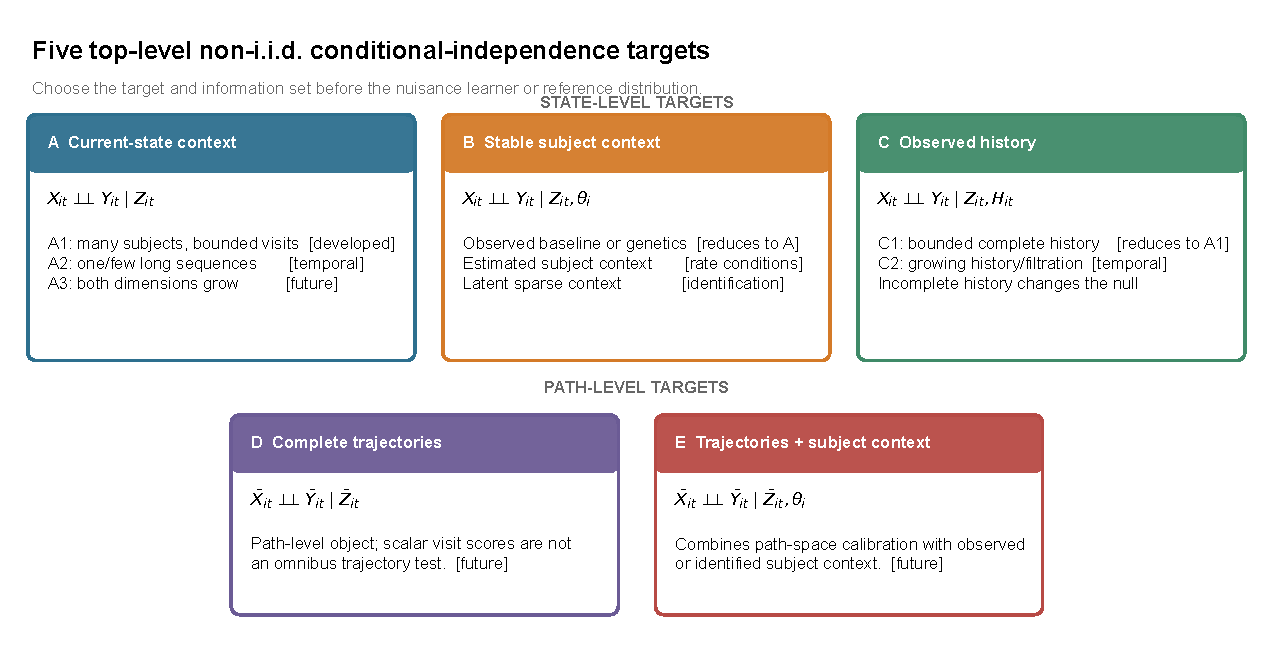
\includegraphics[width=\textwidth]{figure1_taxonomy.pdf}
\caption{Five top-level non-i.i.d. conditional-independence targets. A1--A3 and C1--C2 are
inferential regimes within Cases A and C, respectively, not additional top-level cases.
Blue and green subcases are developed or reducible to the subject-score construction under
the stated information conditions; temporal, latent, and trajectory-level branches require
additional identification or reference-distribution theory.}
\label{fig:taxonomy}
\end{figure}

% ============================================================
\section{Residual-score framework for Cases A--C}

\subsection{Many-subject data and the expanded conditioning set}

Let $i=1,\ldots,N$ index independent subjects and let $t=1,\ldots,m_i$ index
repeated visits within subject $i$. We observe
\[
\mathcal O_i=\{(X_{it},Y_{it},Z_{it}):t=1,\ldots,m_i\}.
\]
The vectors $\mathcal O_1,\ldots,\mathcal O_N$ are assumed independent, while arbitrary
serial or exchangeable dependence is allowed within each $\mathcal O_i$ unless a more
specific assumption is imposed.

The primary developed regime is A1: $N$ independent subjects and a bounded or suitably
controlled number of observations per subject. The notation $Z_{it}$ below denotes the
\emph{complete observed conditioning vector} required by the scientific question. It can be
replaced by $(Z_{it},\theta_i)$ in observed-Case B or by $(Z_{it},H_{it})$ in multi-subject
Case C1. This reduction is valid only when the added information is observed without outcome
leakage and has manageable dimension.

The baseline hypothesis is the visit-level, population-level conditional independence
statement
\begin{equation}
H_0^{\mathrm{pop}}:\quad
X_{it}\indep Y_{it}\mid Z_{it},
\qquad t=1,\ldots,m_i.
\label{eq:pop-null}
\end{equation}
Here ``population-level'' means that subject-specific latent effects are integrated out;
they are not conditioned upon and are not removed through subject-specific BLUPs.

For a prospective question, the aligned target is
\begin{equation}
H_{0,\Delta}^{\mathrm{pop}}:\quad
X_{it}\indep Y_{i,t+\Delta}\mid Z_{it},
\label{eq:prospective-null}
\end{equation}
where $\Delta$ is a pre-specified forecast horizon and $Z_{it}$ contains only information
available at the origin time. The same subject-score construction applies after replacing
$Y_{it}$ by its aligned future outcome. This formulation turns biomarker or sensor evaluation
into a question about information added beyond an explicit reference set.

Time, calendar day, baseline covariates, treatment, environmental variables, and relevant
history should be included in $Z_{it}$ whenever they are scientifically required. This is
important because the interpretation of \eqref{eq:pop-null} is always relative to the chosen
conditioning information.

The present theorem is aimed at many independent subjects with a moderate number of repeated
observations per subject. Very long, high-frequency sequences require an A2 or A3 method that
combines explicit temporal dependence control with cluster-level inference; pre-specified
daily or session summaries may be scientifically useful, but do not by themselves prove the
required conditional-independence statement.

\subsection{Population conditional means and the GCM target}

Define
\[
f_0(z)=\E(X_{it}\mid Z_{it}=z),
\qquad
g_0(z)=\E(Y_{it}\mid Z_{it}=z),
\]
and the marginal residuals
\[
\varepsilon_{it}=X_{it}-f_0(Z_{it}),
\qquad
\xi_{it}=Y_{it}-g_0(Z_{it}).
\]
Let $w_{it}\geq 0$ denote pre-specified within-subject weights satisfying
\[
\sum_{t=1}^{m_i}w_{it}=1.
\]
The equal-subject choice is $w_{it}=m_i^{-1}$. Define the oracle subject score
\begin{equation}
S_i=\sum_{t=1}^{m_i}w_{it}\varepsilon_{it}\xi_{it}.
\label{eq:oracle-score}
\end{equation}
The corresponding population parameter is
\begin{equation}
\rho=\E(S_i)
=\E\left[\sum_{t=1}^{m_i}w_{it}
\{X_{it}-f_0(Z_{it})\}\{Y_{it}-g_0(Z_{it})\}\right].
\label{eq:rho}
\end{equation}
Under \eqref{eq:pop-null}, each same-visit conditional covariance is zero and hence
$\rho=0$.

\begin{remark}[What is and is not tested]
Conditional independence implies $\rho=0$, but the converse does not hold in general.
The scalar GCM is therefore a valid conditional-independence test with power against
alternatives for which the weighted expected conditional covariance is non-zero. Richer
transformations or multivariate scores are needed to detect conditional dependence that
has zero residual covariance.
\end{remark}

\begin{remark}[Equal-subject versus equal-visit targets]
The choice $w_{it}=m_i^{-1}$ gives each subject equal total weight. An equal-visit target
can instead be constructed by weighting subjects proportionally to $m_i$. If cluster size is
informative, the two targets differ scientifically and must not be treated as interchangeable.
\end{remark}

% ============================================================
\section{Procedure for Case A1 and reducible Cases B and C}

\subsection{Testing target}

After constructing the scientifically complete observed context, write it as $Z_{it}$ and
test
\texorpdfstring{$H_0:X_{it}\indep Y_{it}\mid Z_{it}$}
{H0: X independent of Y given Z}.
The same algorithm is therefore used for A1, for Case B with observed $\theta_i$, and for
multi-subject Case C1 with complete finite $H_{it}$. What changes is the meaning and content of
$Z_{it}$, not the score formula.

\subsection{Population-level nuisance estimation}

Estimate $f_0$ and $g_0$ with flexible regression procedures that account for repeated
measurements during fitting. GAMMs are one option, but the target of prediction must remain
$\E(X_{it}\mid Z_{it})$ and $\E(Y_{it}\mid Z_{it})$.

For a Gaussian identity-link GAMM \cite{wood2017}, population-level predictions normally exclude the
subject-specific BLUP. For a nonlinear link, simply omitting the random effect on the linear
predictor scale does not generally equal the marginal mean. The marginal prediction should
then integrate over the fitted random-effect distribution.

\subsection{Cluster-cross-fitted procedure}

\fbox{\begin{minipage}{0.94\textwidth}
\textbf{Procedure 1: Cluster-robust marginal GCM}
\begin{enumerate}[leftmargin=*,label=\arabic*.]
\item Split the $N$ subjects into $K$ folds $I_1,\ldots,I_K$. All visits from one subject
must remain in the same fold.

\item For fold $k$, use subjects in $I_k^c$ to fit
\[
\widehat f^{(-k)}(z)\approx \E(X\mid Z=z),
\qquad
\widehat g^{(-k)}(z)\approx \E(Y\mid Z=z).
\]
If a supervised neural-network embedding is part of $X$, train the network, choose the
embedding layer, and perform all dimension reduction using training subjects only.

\item For each held-out subject $i\in I_k$, compute population-level residuals
\[
\widehat\varepsilon_{it}
=X_{it}-\widehat f^{(-k)}(Z_{it}),
\qquad
\widehat\xi_{it}
=Y_{it}-\widehat g^{(-k)}(Z_{it}).
\]
Do not include held-out subject-specific BLUPs in a marginal analysis.

\item Construct the held-out subject score
\[
\widehat S_i
=\sum_{t=1}^{m_i}w_{it}
\widehat\varepsilon_{it}\widehat\xi_{it}.
\]

\item Pool the cross-fitted scores and compute
\[
\overline S_N=\frac1N\sum_{i=1}^N\widehat S_i,
\qquad
\widehat\sigma_N^2
=\frac1N\sum_{i=1}^N(\widehat S_i-\overline S_N)^2.
\]

\item Form
\begin{equation}
T_N=\frac{\sqrt N\,\overline S_N}{\widehat\sigma_N}.
\label{eq:test-statistic}
\end{equation}
Reject the two-sided null at level $\alpha$ when
$|T_N|>z_{1-\alpha/2}$.
\end{enumerate}
\end{minipage}}

\subsection{Interpretation}

The first-stage regressions remove the population-level dependence of $X$ and $Y$ on $Z$.
The subject score aggregates all visit-level residual products within one independent cluster.
The denominator estimates the variance of the complete subject score, and therefore includes
all within-subject covariance terms automatically.

This differs fundamentally from treating all $M=\sum_i m_i$ visits as independent and using
$\sqrt M$ scaling. The effective asymptotic unit is the subject, so the basic scaling is
$\sqrt N$.

\subsection{Several markers and a global multiplier test}

For markers $X^{(1)},\ldots,X^{(p)}$, let $\widehat S_{ij}$ be the cross-fitted subject
score for marker $j$, with mean $\overline S_j$ and empirical standard deviation
$\widehat\sigma_j$. The marker statistic is
\[
T_j=\frac{\sqrt N\,\overline S_j}{\widehat\sigma_j},
\qquad j=1,\ldots,p,
\]
and the global statistic is $M=\max_j|T_j|$. For multiplier draw $b$, generate independent
standard normal variables,
\[
e_i^{(b)}\sim N(0,1),\qquad i=1,\ldots,N,
\]
and calculate
\[
T_j^{*(b)}=
\frac{1}{\sqrt N\,\widehat\sigma_j}
\sum_{i=1}^N e_i^{(b)}(\widehat S_{ij}-\overline S_j),
\qquad
M^{*(b)}=\max_j|T_j^{*(b)}|.
\]
With $B$ multiplier draws, the empirical global $p$-value is
\[
\widehat p_{\mathrm{global}}
=\frac{1+\sum_{b=1}^B\mathbf 1\{M^{*(b)}\geq M\}}{B+1}.
\]
The same multiplier is applied to all markers within a subject, thereby preserving their
estimated dependence. In the application, the global test is primary and normal-reference
marker tests are adjusted by Holm's method.

% ============================================================
\section{Theoretical framework for Case A1}

\subsection{Notation for cross-fitted prediction errors}

For subject $i$ in fold $k(i)$, define
\[
\Delta^f_{it}
=\widehat f^{(-k(i))}(Z_{it})-f_0(Z_{it}),
\qquad
\Delta^g_{it}
=\widehat g^{(-k(i))}(Z_{it})-g_0(Z_{it}).
\]
Then
\begin{equation}
\widehat\varepsilon_{it}\widehat\xi_{it}
=
\varepsilon_{it}\xi_{it}
-\varepsilon_{it}\Delta^g_{it}
-\xi_{it}\Delta^f_{it}
+\Delta^f_{it}\Delta^g_{it}.
\label{eq:cluster-decomposition-observation}
\end{equation}
At subject level,
\begin{equation}
\widehat S_i
=S_i-C_{g,i}-C_{f,i}+B_i,
\label{eq:cluster-decomposition}
\end{equation}
where
\[
C_{g,i}=\sum_t w_{it}\varepsilon_{it}\Delta^g_{it},
\qquad
C_{f,i}=\sum_t w_{it}\xi_{it}\Delta^f_{it},
\qquad
B_i=\sum_t w_{it}\Delta^f_{it}\Delta^g_{it}.
\]

\subsection{High-level assumptions}

\begin{assumption}[Independent clusters]
The subject vectors $\mathcal O_1,\ldots,\mathcal O_N$ are independent. They may be
non-identically distributed in a triangular array, provided the following moment and
variance conditions hold uniformly.
\end{assumption}

\begin{assumption}[Weights and cluster size]
The weights are nonnegative and satisfy $\sum_t w_{it}=1$. Either
$\max_i m_i\leq m_{\max}<\infty$, or growing clusters satisfy a Lindeberg condition that
prevents a single subject from dominating the total score.
\end{assumption}

\begin{assumption}[Oracle centering]
For every visit,
\[
\E(\varepsilon_{it}\mid Z_{it})=0,
\qquad
\E(\xi_{it}\mid Z_{it})=0.
\]
Under the null, $X_{it}\indep Y_{it}\mid Z_{it}$ and therefore
$\E(\varepsilon_{it}\xi_{it}\mid Z_{it})=0$.
\end{assumption}

\begin{assumption}[Oracle cluster CLT]
\label{ass:oracle-clt}
For some $\delta>0$,
\[
\sup_i\E|S_i-\E S_i|^{2+\delta}<\infty,
\]
and
\[
\sigma_N^2=\frac1N\sum_{i=1}^N\Var(S_i)
\longrightarrow \sigma^2\in(0,\infty).
\]
The corresponding Lindeberg condition holds. For identically distributed clusters this
reduces to $0<\Var(S_i)<\infty$ plus a suitable $2+\delta$ moment.
\end{assumption}

\begin{assumption}[Cluster cross-fitting]
For every held-out cluster $i$, the functions
$\widehat f^{(-k(i))}$ and $\widehat g^{(-k(i))}$ are estimated without using any
observation from subject $i$. Conditional on the corresponding fold-specific training data,
the prediction errors at a
held-out visit are functions of the held-out $Z_{it}$, not of held-out $X_{it}$ or $Y_{it}$.
\end{assumption}

\begin{assumption}[Product-rate condition]
Define the cluster-weighted mean squared prediction errors
\[
A_f=\frac1N\sum_{i=1}^N\sum_{t=1}^{m_i}w_{it}(\Delta^f_{it})^2,
\qquad
A_g=\frac1N\sum_{i=1}^N\sum_{t=1}^{m_i}w_{it}(\Delta^g_{it})^2.
\]
Assume
\begin{equation}
A_fA_g=\op(N^{-1}).
\label{eq:product-rate}
\end{equation}
Equivalently, if $r_f=A_f^{1/2}$ and $r_g=A_g^{1/2}$ are empirical RMSEs, then
$\sqrt N\,r_fr_g=\op(1)$.
\end{assumption}

\begin{assumption}[Cluster-weighted cross-term control]
\label{ass:cross-term}
Let $n_k=|I_k|$ and let $\calT_k$ denote the observations from subjects outside fold $I_k$,
together with the fold assignment. For fixed $K$, assume
\begin{align}
B_{g,k}^{\mathrm{cl}}
&=
\frac1{n_k}\sum_{i\in I_k}
\E\left[
\left(\sum_t w_{it}\varepsilon_{it}\Delta^g_{it}\right)^2
\middle|\calT_k
\right]
\quad
\max_{k\leq K}B_{g,k}^{\mathrm{cl}}=\op(1),
\label{eq:Bg-cluster}\\
B_{f,k}^{\mathrm{cl}}
&=
\frac1{n_k}\sum_{i\in I_k}
\E\left[
\left(\sum_t w_{it}\xi_{it}\Delta^f_{it}\right)^2
\middle|\calT_k
\right]
\quad
\max_{k\leq K}B_{f,k}^{\mathrm{cl}}=\op(1).
\label{eq:Bf-cluster}
\end{align}
\end{assumption}

\begin{remark}[A sufficient covariance-operator condition]
Let $\bfDelta_i^g=(\Delta^g_{i1},\ldots,\Delta^g_{im_i})^\top$,
$W_i=\operatorname{diag}(w_{i1},\ldots,w_{im_i})$, and let
$\Omega_i^X$ denote the conditional or unconditional covariance matrix of
$(\varepsilon_{i1},\ldots,\varepsilon_{im_i})^\top$ under the conditioning used in the proof.
Then a sufficient version of \eqref{eq:Bg-cluster}, applied uniformly over the fixed folds, is
\[
\max_{k\leq K}\frac1{n_k}\sum_{i\in I_k}
(\bfDelta_i^g)^\top W_i\Omega_i^XW_i\bfDelta_i^g
=\op(1),
\]
with the analogous condition for $f$. If the operator norms of $\Omega_i^X$ and
$\Omega_i^Y$ are uniformly bounded, ordinary cluster-weighted $L_2$ consistency is sufficient
for these two conditions.
\end{remark}

\begin{assumption}[Variance consistency]
\label{ass:variance}
The estimated subject scores satisfy
\[
\frac1N\sum_{i=1}^N(\widehat S_i-S_i)^2=\op(1),
\]
and a law of large numbers holds for $S_i^2$. Consequently,
\[
\widehat\sigma_N^2-\frac1N\sum_i(S_i-\overline S_N^0)^2=\op(1),
\]
where $\overline S_N^0=N^{-1}\sum_iS_i$.
\end{assumption}

\subsection{Null theorem and proof roadmap}

\begin{theorem}[Proposed null validity of cluster GCM]
Under Assumptions 4.1--4.8 and $H_0^{\mathrm{pop}}$, the statistic in
\eqref{eq:test-statistic} satisfies
\[
T_N\xrightarrow{d}N(0,1).
\]
If all assumptions hold uniformly over a class of null distributions, then the convergence is
uniform and the resulting test has uniformly asymptotic level $\alpha$ over that class.
\end{theorem}

\begin{proof}[Proof roadmap]
Using \eqref{eq:cluster-decomposition},
\begin{align}
\sqrt N\,\overline S_N
&=
\frac1{\sqrt N}\sum_{i=1}^NS_i
-
\frac1{\sqrt N}\sum_{i=1}^NC_{g,i}
-
\frac1{\sqrt N}\sum_{i=1}^NC_{f,i}
+
\frac1{\sqrt N}\sum_{i=1}^NB_i.
\label{eq:cluster-numerator-decomp}
\end{align}
The proof consists of four steps.

\textbf{Step 1: Oracle cluster CLT.}
Under the null, $\E S_i=0$. Assumption~\ref{ass:oracle-clt} gives
\[
\frac{N^{-1/2}\sum_iS_i}{\sigma_N}\xrightarrow{d}N(0,1).
\]
Within-subject dependence is entirely contained in $S_i$ and does not violate the CLT because
subjects are independent.

\textbf{Step 2: Product-bias term.}
By Cauchy--Schwarz and $\sum_t w_{it}=1$,
\begin{align*}
\left|\frac1{\sqrt N}\sum_iB_i\right|
&\leq
\sqrt N
\left\{
\frac1N\sum_{i,t}w_{it}(\Delta^f_{it})^2
\right\}^{1/2}
\left\{
\frac1N\sum_{i,t}w_{it}(\Delta^g_{it})^2
\right\}^{1/2}\\
&=\sqrt N(A_fA_g)^{1/2}=\op(1).
\end{align*}

\textbf{Step 3: Two first-order cross terms.}
For each fold $k$, cluster cross-fitting ensures that, conditional on $\calT_k$, held-out
nuisance functions do not depend on held-out responses. Since
$\E(\varepsilon_{it}\mid Z_{it})=0$ and
$\E(\xi_{it}\mid Z_{it})=0$, each cross term is centred after conditioning on the
appropriate fold-specific training information. Subjects within $I_k$ are conditionally
independent given $\calT_k$, and Assumption~\ref{ass:cross-term} gives
\[
\frac1{\sqrt{n_k}}\sum_{i\in I_k}C_{g,i}=\op(1),
\qquad
\frac1{\sqrt{n_k}}\sum_{i\in I_k}C_{f,i}=\op(1)
\]
by conditional Chebyshev's inequality. Summing the fixed number of folds with weights
$\sqrt{n_k/N}$ yields the two $N^{-1/2}$ results required in
\eqref{eq:cluster-numerator-decomp}. This foldwise argument avoids conditioning jointly on
overlapping training samples.

\textbf{Step 4: Studentisation.}
Assumption~\ref{ass:variance} implies
$\widehat\sigma_N^2\to_{\mathbb P}\sigma^2$.
Slutsky's theorem completes the proof.
\end{proof}

\subsection{Alternative theorem and power}

Under a general alternative, define
\[
\rho_N=\frac1N\sum_{i=1}^N\E(S_i),
\qquad
\sigma_{N,A}^2=\frac1N\sum_{i=1}^N\Var(S_i).
\]
For identically distributed clusters, $\rho_N=\rho$ and
$\sigma_{N,A}^2=\Var(S_i)$.

\begin{theorem}[Proposed asymptotic linearity under alternatives]
Assume cluster cross-fitting and the analogues of Assumptions 4.4--4.8 for the centred
oracle scores $S_i-\E S_i$. Then
\[
\frac{\sqrt N(\overline S_N-\rho_N)}{\widehat\sigma_N}
\xrightarrow{d}N(0,1).
\]
Consequently, fixed alternatives with $\rho\neq0$ are detected consistently. Under local
alternatives $\rho_N=c/\sqrt N$, the limiting distribution is normal with mean
$c/\sigma$ and variance one.
\end{theorem}

\begin{remark}[Why cross-fitting is more important under alternatives]
Without splitting, the regression estimate of $g_0$ is a function of the same $Y$ values used
in the test. Under the null, conditional independence may provide a same-sample centering
argument. Under an alternative, $\E(\varepsilon\mid Y,Z)$ need not vanish, so the first-order
cross term is no longer automatically centred. Cluster cross-fitting restores centering through
$\E(\varepsilon\mid Z)=0$ and $\E(\xi\mid Z)=0$, properties that hold under both the null
and the alternative.
\end{remark}

% ============================================================
\section{Score, quasi-score, and exponential-family extensions}

\subsection{General conditionally centred score}

Let $q_0(Y,Z)$ be any square-integrable transformation satisfying
\begin{equation}
\E\{q_0(Y,Z)\mid Z\}=0.
\label{eq:q-centering}
\end{equation}
Define the oracle score-GCM contribution
\[
R^q_{it}=\{X_{it}-f_0(Z_{it})\}q_0(Y_{it},Z_{it}),
\]
and the subject score
\[
S_i^q=\sum_tw_{it}R^q_{it}.
\]
Under $X_{it}\indep Y_{it}\mid Z_{it}$,
\[
\E(R^q_{it}\mid Z_{it})
=\E(\varepsilon_{it}\mid Z_{it})
\E\{q_0(Y_{it},Z_{it})\mid Z_{it}\}=0.
\]
Thus a conditionally centred score may replace the ordinary $Y$ residual.

Let $\widehat q_{it}$ be a cross-fitted estimate and define
\[
\Delta^q_{it}=\widehat q_{it}-q_0(Y_{it},Z_{it}).
\]
The estimated product has the exact expansion
\begin{align}
\{X_{it}-\widehat f(Z_{it})\}\widehat q_{it}
&=
\varepsilon_{it}q_{0,it}
-\Delta^f_{it}q_{0,it}
+\varepsilon_{it}\Delta^q_{it}
-\Delta^f_{it}\Delta^q_{it}.
\label{eq:q-decomp}
\end{align}
Define
\[
A_q=\frac1N\sum_{i,t}w_{it}(\Delta^q_{it})^2.
\]
The direct analogue of the GCM product-rate condition is
\begin{equation}
A_fA_q=\op(N^{-1}).
\label{eq:q-product-rate}
\end{equation}
The corresponding cluster cross-term conditions replace $\xi$ by $q_0$ and
$\Delta^g$ by $\Delta^q$ in \eqref{eq:Bg-cluster}--\eqref{eq:Bf-cluster}.

\subsection{Exponential-family outcome}

Suppose the conditional density of $Y$ is
\[
p(y\mid Z)
=
\exp\left[
\frac{y\theta(Z)-b\{\theta(Z)\}}{a(\phi)}+c(y,\phi)
\right].
\]
Then
\[
\mu_0(Z)=\E(Y\mid Z)=b'\{\theta(Z)\},
\qquad
\Var(Y\mid Z)=a(\phi)b''\{\theta(Z)\}.
\]
The score for the natural parameter is
\begin{equation}
q_0^{\mathrm{can}}(Y,Z)
=\frac{Y-\mu_0(Z)}{a(\phi)}.
\label{eq:canonical-score}
\end{equation}
When $a(\phi)$ is known or is a global bounded scale, it can be omitted without changing the
studentised test. With
\[
\widehat q^{\mathrm{can}}(Y,Z)=Y-\widehat\mu(Z),
\]
we have
\[
\Delta^q(Z)=\mu_0(Z)-\widehat\mu(Z),
\]
which is a function of $Z$ and training data only. Therefore
\[
A_q
=
\frac1N\sum_{i,t}w_{it}
\{\widehat\mu(Z_{it})-\mu_0(Z_{it})\}^2,
\]
and the required condition is exactly
\begin{equation}
A_fA_\mu=\op(N^{-1}).
\label{eq:expfam-rate}
\end{equation}
This is the cleanest exponential-family extension: the null and alternative proof structures
are the same as for the ordinary GCM.

\begin{remark}[Rates]
If $r_f=A_f^{1/2}=\Op(N^{-\alpha})$ and
$r_\mu=A_\mu^{1/2}=\Op(N^{-\beta})$, then
\eqref{eq:expfam-rate} requires $\alpha+\beta>1/2$.
If the outcome mean is estimated by a correctly specified finite-dimensional GLM,
$r_\mu=\Op(N^{-1/2})$, so consistency of the $X$ regression may be sufficient.
If both sides are nonparametric with comparable difficulty, each RMSE typically needs to be
$o_{\mathbb P}(N^{-1/4})$.
\end{remark}

\subsection{Quasi-score}

A general quasi-score can be written as
\begin{equation}
q_0^{\mathrm{Q}}(Y,Z)
=w_0(Z)\{Y-\mu_0(Z)\},
\label{eq:quasi-score}
\end{equation}
where $w_0(Z)$ is a bounded, pre-specified, or externally estimated weight. Since
$\E(q_0^{\mathrm{Q}}\mid Z)=0$, the null proof remains valid. If $w_0$ is fixed and bounded,
then
\[
A_q\lesssim A_\mu
\]
and the same product-rate condition applies.

The classical quasi-likelihood choice is
\[
w_0(Z)=\frac{\partial\mu_0(Z)/\partial\eta}
{\Var(Y\mid Z)},
\]
but full distributional correctness is not required for centering if the mean model is correct
and the weight is a function of $Z$ only.

\subsection{Pearson residuals and estimated weights}

The Pearson residual is
\[
q_0^{\mathrm{P}}(Y,Z)
=\frac{Y-\mu_0(Z)}{\sigma_0(Z)}.
\]
It is conditionally centred when $\sigma_0(Z)>0$. If $\sigma_0$ is known or treated as a fixed
bounded weight, the theory is the same as the quasi-score theory.

If $\sigma_0$ is estimated,
\begin{align*}
\widehat q^{\mathrm{P}}-q_0^{\mathrm{P}}
&=
\frac{\mu_0-\widehat\mu}{\widehat\sigma}
+(Y-\mu_0)
\left(\frac1{\widehat\sigma}-\frac1{\sigma_0}\right).
\end{align*}
The second term depends on $Y$. Under the null, conditional independence can still help
centre the corresponding cross term. Under a general alternative, however, independent
sample splitting alone does not make this term mean zero because
$\E\{\varepsilon(Y-\mu_0)\mid Z\}$ is precisely a conditional covariance. A separate rate,
Taylor expansion, or a score orthogonalised with respect to the variance nuisance is then
required.

\subsection{Likelihood and deviance transformations}

A raw log-likelihood contribution $\ell(Y;\theta(Z))$ and a deviance residual are generally
not conditionally mean zero. They cannot be inserted into the GCM without centering. A valid
transformation is
\[
q_0^{\ell}(Y,Z)
=
\ell\{Y;\theta_0(Z)\}
-
\E[\ell\{Y;\theta_0(Z)\}\mid Z].
\]
This introduces additional nuisance functions and typically creates $Y$-dependent estimation
errors. It is therefore less attractive than the canonical or fixed-weight quasi-score for a
first theoretical development.

\subsection{Distributional score vector}

To investigate whether $X$ is related to different aspects of the conditional distribution of
$Y$, one may use a vector of centred scores, for example
\[
q_{1,0}(Y,Z)=Y-\mu_0(Z),
\qquad
q_{2,0}(Y,Z)=\{Y-\mu_0(Z)\}^2-\Var(Y\mid Z).
\]
The resulting multivariate GCM can test association with the conditional mean and dispersion
simultaneously. Inference then follows from a fixed-dimensional Wald argument or a
high-dimensional maximum-statistic argument.

% ============================================================
\section{Sample splitting and cross-fitting}

\subsection{Why splitting must be by subject}

All visits from one subject must be kept in the same fold. Visit-level random splitting leaks
subject-specific information between the training and test sets, invalidates the interpretation
of an out-of-sample score, and can make the nuisance estimators dependent on the held-out
cluster score.

Cluster splitting also avoids a subtle strengthening of the null. If $\widehat g$ is estimated
using all $Y$ values from subject $i$, controlling
$\varepsilon_{it}\{g(Z_{it})-\widehat g(Z_{it})\}$ may require information about
$\E(\varepsilon_{it}\mid\mathbf Y_i,\mathbf Z_i)$ and can therefore implicitly require
cross-time or trajectory-level conditional independence. Leaving the entire cluster out avoids
this issue for the visit-level target.

\subsection{Recommended \texorpdfstring{$K$}{K}-fold procedure}

For $k=1,\ldots,K$:
\begin{enumerate}[leftmargin=*]
\item Fit all nuisance models on $I_k^c$.
\item Pre-specify preprocessing, neural-network weights, embedding extraction, basis
estimation, variable selection, and tuning parameters using the corresponding analysis set.
\item Predict population-level quantities for subjects in $I_k$.
\item Compute held-out visit contributions and one score per held-out subject.
\end{enumerate}
Pool the $N$ subject scores and studentise once at the end. Repeated cross-fitting may be used
to reduce random fold variability, but the repetition scheme must be included in the bootstrap
or variance calculation if scores are averaged across repeated splits.

\subsection{What cross-fitting solves and what it does not}

Cross-fitting solves the dependence between nuisance fitting and held-out score construction.
It does not by itself guarantee small prediction error, correct marginalisation over random
effects, or identification of a latent subject effect. Product-rate and cross-term conditions
remain necessary.

% ============================================================
\section{Relevant theory of the original GCM}

This section records the original GCM results that the repeated-measures proof should mirror.

\subsection{Original univariate statistic}

For i.i.d. observations $(X_i,Y_i,Z_i)$, define
\[
f_0(z)=\E(X\mid Z=z),
\qquad
g_0(z)=\E(Y\mid Z=z),
\]
\[
\varepsilon_i=X_i-f_0(Z_i),
\qquad
\xi_i=Y_i-g_0(Z_i),
\]
and
\[
R_i=\{X_i-\widehat f(Z_i)\}\{Y_i-\widehat g(Z_i)\}.
\]
The statistic is
\[
T_n
=
\frac{n^{-1/2}\sum_iR_i}
{\left[n^{-1}\sum_iR_i^2-(n^{-1}\sum_iR_i)^2\right]^{1/2}}.
\]

Define
\begin{align*}
A_f&=\frac1n\sum_i\{f_0(Z_i)-\widehat f(Z_i)\}^2,
&
A_g&=\frac1n\sum_i\{g_0(Z_i)-\widehat g(Z_i)\}^2,\\
B_f&=\frac1n\sum_i\{f_0(Z_i)-\widehat f(Z_i)\}^2
\E(\xi_i^2\mid Z_i),
&
B_g&=\frac1n\sum_i\{g_0(Z_i)-\widehat g(Z_i)\}^2
\E(\varepsilon_i^2\mid Z_i).
\end{align*}

\subsection{Theorem 6: null validity}

The pointwise result assumes
\[
A_fA_g=\op(n^{-1}),
\qquad
B_f=\op(1),
\qquad
B_g=\op(1),
\qquad
0<\E(\varepsilon^2\xi^2)<\infty.
\]
Then
\[
\sup_t|\Pp(T_n\leq t)-\Phi(t)|\to0.
\]
The uniform result additionally requires, over a null class $\mathcal P$,
\[
\inf_{P\in\mathcal P}\E_P(\varepsilon_P^2\xi_P^2)>0,
\qquad
\sup_{P\in\mathcal P}\E_P|\varepsilon_P\xi_P|^{2+\eta}<\infty,
\]
and uniform versions of the prediction-error conditions.

The key numerator expansion is
\begin{align}
\frac1{\sqrt n}\sum_iR_i
&=
\frac1{\sqrt n}\sum_i\varepsilon_i\xi_i
+
\frac1{\sqrt n}\sum_i\{f_0(Z_i)-\widehat f(Z_i)\}
\{g_0(Z_i)-\widehat g(Z_i)\} \nonumber\\
&\quad+
\frac1{\sqrt n}\sum_i\varepsilon_i\{g_0(Z_i)-\widehat g(Z_i)\}
+
\frac1{\sqrt n}\sum_i\xi_i\{f_0(Z_i)-\widehat f(Z_i)\}.
\label{eq:original-gcm-decomp}
\end{align}
The four proof components are:
\begin{enumerate}[leftmargin=*]
\item an i.i.d. CLT for $n^{-1/2}\sum_i\varepsilon_i\xi_i$;
\item Cauchy--Schwarz for the product-bias term;
\item null conditional mean-zero arguments for the two cross terms, controlled by $B_f,B_g$;
\item expansion of $R_i^2-\varepsilon_i^2\xi_i^2$, a law of large numbers, and Slutsky's
lemma for denominator consistency.
\end{enumerate}

The same-sample null argument uses
\[
\E(\varepsilon_i\mid Y^{(n)},Z^{(n)})=0,
\qquad
\E(\xi_i\mid X^{(n)},Z^{(n)})=0,
\]
which follows from i.i.d. sampling and $X\indep Y\mid Z$.

\subsection{Theorem 8: alternatives and power}

Define
\[
\rho_P=\E_P\{\Cov_P(X,Y\mid Z)\}=\E_P(\varepsilon_P\xi_P),
\qquad
\sigma_P^2=\Var_P(\varepsilon_P\xi_P).
\]
When $\widehat f$ and $\widehat g$ are trained on an auxiliary sample independent of the test
sample, the centred statistic satisfies
\[
\frac{\tau_N^{(n)}-\sqrt n\rho_P}{\tau_D^{(n)}}
\xrightarrow{d}N(0,1),
\qquad
\tau_D^{(n)}\to_{\mathbb P}\sigma_P,
\]
under analogues of Theorem 6's conditions for
$\varepsilon_P\xi_P-\E_P(\varepsilon_P\xi_P)$.
Thus the empirical residual covariance estimates $\rho_P$ at the root-$n$ rate.

Auxiliary-sample training is used because, under an alternative,
$\E(\varepsilon\mid Y,Z)$ and $\E(\xi\mid X,Z)$ need not vanish. Given independent training
data and $Z$, however, the nuisance errors are fixed functions of $Z$, and
\[
\E\{\varepsilon\Delta_g(Z)\mid Z,\calT\}=0,
\qquad
\E\{\xi\Delta_f(Z)\mid Z,\calT\}=0.
\]

\subsection{Theorem 9: multivariate and high-dimensional GCM}

For $X\in\R^{d_X}$ and $Y\in\R^{d_Y}$, construct pairwise statistics $T_{jk}$ and define
\[
S_n=\max_{j\leq d_X,\,k\leq d_Y}|T_{jk}|.
\]
The reference distribution is the maximum of a centred Gaussian vector with covariance
estimated from the empirical correlations of pairwise residual-product vectors.

The high-dimensional theorem requires:
\begin{enumerate}[leftmargin=*]
\item sub-exponential or sufficiently high-order moment conditions for every
$\varepsilon_j\xi_k$;
\item non-degenerate pairwise variances;
\item a high-dimensional CLT rate such as
$C_n^2\{\log(dn)\}^7/n$ tending to zero sufficiently fast;
\item the strengthened product-rate condition
\[
\max_{j,k}A_{f,j}A_{g,k}
=\op\{n^{-1}(\log d)^{-2}\};
\]
\item maximal residual and prediction-error conditions controlling all cross terms
simultaneously.
\end{enumerate}
The proof combines high-dimensional Gaussian approximation, maximal inequalities for the
nuisance terms, sup-norm covariance estimation, and Gaussian anti-concentration.

\subsection{Theorem 11: kernel ridge regression}

The kernel-ridge section verifies Theorem 6's abstract prediction requirements for a concrete
regression method. If $f_0,g_0$ belong to a reproducing-kernel Hilbert space, conditional
variances are bounded, residual-product moments are controlled, RKHS norms are uniformly
bounded, and the kernel eigenvalue tails satisfy
\[
\lim_{\lambda\downarrow0}
\sup_{P\in\mathcal P}
\sum_{j=1}^{\infty}\min(\mu_{P,j},\lambda)=0,
\]
then the KRR-based GCM is pointwise, and under uniform assumptions uniformly, asymptotically
normal.

The proof derives a KRR prediction bound by decomposing error into a variance term and a
regularisation-bias term, controls empirical kernel eigenvalues through population eigenvalues,
chooses $\lambda$ to make the prediction MSE $o(n^{-1/2})$, verifies
$A_fA_g=\op(n^{-1})$ and $B_f,B_g=\op(1)$, and then invokes Theorem 6.

% ============================================================
\section{Case B: observed, estimated, and latent subject context}

\subsection{Observed context reduces to Case A}

When $\theta_i$ is observed independently of the tested outcomes, define
$Z_{it}^{\star}=(Z_{it},\theta_i)$ and apply the A1 cluster-score procedure. Time-invariant
genetic information is a typical example: its lack of temporal variation does not prevent it
from serving as a conditioning variable. It contributes between-subject information and must
remain inside each subject's fold.

When $\theta_i$ is estimated, write $\widehat\theta_i=\theta_i+r_i$. Treating
$\widehat\theta_i$ as if it were observed is justified only if the induced nuisance errors
satisfy the same product-rate and cross-term conditions as the other regressions. Estimation
from auxiliary information independent of the tested innovations is substantially easier to
analyse than estimation from the same $X$ and $Y$ trajectories. The latter can create both
non-vanishing measurement error and outcome leakage.

\subsection{A different scientific target}

The subject-conditional null
\begin{equation}
H_0^{\mathrm{sub}}:\quad
X_{it}\indep Y_{it}\mid Z_{it},U_i
\label{eq:subject-null}
\end{equation}
asks whether same-visit deviations remain associated after conditioning on a stable latent
subject characteristic $U_i$. This is not the same question as the population-level null.
A shared random effect can violate the population null while \eqref{eq:subject-null} remains
true.

\subsection{Latent-effect identification}

If $U_i$ is unobserved, \eqref{eq:subject-null} is generally not nonparametrically identified
from the observed distribution. Its meaning depends on the chosen latent-variable model,
random-effect distribution, and random-effect design. The test is therefore necessarily more
model-dependent than the marginal cluster GCM.

\subsection{Finite visits and irreducible prediction error}

Consider the random-intercept model
\[
X_{it}=b_i+e_{it},
\qquad
b_i\sim N(0,\tau^2),
\qquad
e_{it}\sim N(0,\sigma^2).
\]
Even when $\tau^2$ and $\sigma^2$ are known, the posterior mean predictor based on $m$ visits
has prediction risk
\[
\E\left[\{b_i-\E(b_i\mid X_{i1},\ldots,X_{im})\}^2\right]
=
\frac{\tau^2\sigma^2}{\sigma^2+m\tau^2}.
\]
For fixed $m$, this is bounded away from zero. Increasing the number of subjects estimates the
random-effect distribution more accurately, but does not consistently recover each realised
$b_i$.

\subsection{BLUP shrinkage can create residual dependence}

Suppose
\[
X_{it}=b_i+e^X_{it},
\qquad
Y_{it}=b_i+e^Y_{it},
\]
with conditional independence given $b_i$. If separate BLUPs satisfy
$\widehat b_i^X\approx\lambda_X\overline X_i$ and
$\widehat b_i^Y\approx\lambda_Y\overline Y_i$ with $0<\lambda_X,\lambda_Y<1$, then
\[
X_{it}-\widehat b_i^X
=(1-\lambda_X)b_i+\text{noise},
\]
and similarly for $Y$. The residual product contains
\[
(1-\lambda_X)(1-\lambda_Y)b_i^2,
\]
whose expectation is positive. Thus a subject-conditional null can be falsely rejected because
the latent effect is only partially removed.

\subsection{Why sample splitting is insufficient}

Within-subject splitting can prevent a visit from being used both to estimate $U_i$ and to
form its own residual. It removes self-influence but does not create additional information
about $U_i$. With a bounded number of visits, the latent-effect prediction error remains
non-vanishing and the product of two such errors can induce first-order bias.

If $U_i$ is estimated using other $Y$ visits from the same subject, a same-visit null
may not be enough to centre the cross term. One may implicitly require
\[
\E(\varepsilon^X_{it}\mid\mathbf Y_i,\mathbf Z_i,U_i)=0,
\]
which is closer to a trajectory-level conditional-independence assumption.

\subsection{Dense-visit regime}

A subject-conditional theory becomes more plausible when
\[
N\to\infty,
\qquad
m_{\min}=\min_i m_i\to\infty,
\]
and finite-dimensional random effects are identifiable from the within-subject design.
If
\[
\widehat h_X(U_i)-h_X(U_i)=\Op(m_i^{-1/2}),
\qquad
\widehat h_Y(U_i)-h_Y(U_i)=\Op(m_i^{-1/2}),
\]
then the corresponding mean squared errors are $O(m_i^{-1})$. A generic root-$N$ GCM
product bound requires approximately
\[
\frac{\sqrt N}{m_{\min}}\to0.
\]
This dense-longitudinal regime is not representative of studies with only a few visits per
subject.

\subsection{Recommended interpretation}

For sparse repeated-measures data, the subject-conditional GAMM-residual GCM should be
presented as a model-based sensitivity analysis rather than the primary general theory. The
primary method should target the population-level null and use population predictions plus
cluster-robust inference.

% ============================================================
\section{Case C: bounded and growing observed history}

\subsection{C1: many subjects with bounded histories}

Let $H_{it}$ be a finite vector constructed only from information available before the tested
pair, for example $H_{it}=(X_{i,t-1},Y_{i,t-1})$. For
\[
H_0^C:\quad X_{it}\indep Y_{it}\mid Z_{it},H_{it},
\]
define $Z_{it}^{\star}=(Z_{it},H_{it})$ and apply the subject-cross-fitted procedure. Serial
dependence among visits is retained within $S_i$; no visit-level independence assumption is
introduced. With fixed-dimensional history and independent subjects, this is a reduction to
A1 rather than a separate temporal central limit theorem.

The history must nevertheless be scientifically complete for the stated null. If the true
process contains $X_{i,t-1}\to Y_{it}$ but only $Y_{i,t-1}$ is conditioned on, the fitted test
targets a different hypothesis. Flexible regression cannot compensate for an omitted state
variable.

\subsection{C2: growing history in one or a few long sequences}

For fixed $N$ and $T\to\infty$, subject aggregation does not create an increasing number of
independent scores. The residual products form a time series. Shi's GTCM proposal considers
the predictive null $Y_{t+1}\indep X_t\mid\{\bar Y_t,\bar Z_t\}$ and uses regression
stability plus weak dependence to control the bias created by training nuisance functions on
correlated observations \cite{shi2025}. That argument motivates the A2/C2 branch of the
taxonomy, but it is not supplied by the present $\sqrt N$ theorem. A temporal implementation
would need an explicit long-run variance or martingale/self-normalised reference distribution
and a time-respecting fitting rule.

\subsection{High-dimensional measurements and learned representations}

GAMMs are convenient for smooth low-dimensional context, but the framework is learner-
agnostic. A random forest, boosted model, kernel method, neural regression, or other learner
may replace a GAMM when its out-of-cluster prediction errors satisfy the stated product-rate
and cross-term conditions. For high-dimensional $X$, including images or dense sensor
windows, a representation $\omega(X)$ may be tested instead of the raw object. DNCIT shows
how unsupervised, conditionally unsupervised, or transfer-learned representations can be
combined with a downstream nonparametric CIT when the representation training cannot create
conditional dependence with $Y$ \cite{simnacher2024}. In clustered data, that requirement is
additional to subject-level splitting: any supervised representation selection involving
$Y$ must occur using training subjects only.

This composition changes the detectable alternative and may lose information if the
embedding is not sufficient. It does not turn the scalar residual covariance into an omnibus
test, and it does not yet solve the trajectory-level nulls D or E.

% ============================================================
\section{Simulation study}

\subsection{Objectives and design}

The simulation study had six linked components: a preliminary numerical check, a formal
assessment under the core Case-A1 population null, a broader collection of A1 null settings,
an inferential-unit comparison, a frozen extension isolating the information requirements in
Cases B and C1, and a supplementary gradient for generated-context accuracy and local power.
The original Case-A analyses used three $X$ markers, one continuous $Y$,
subject-level scores, five folds for Design A, and a Gaussian multiplier global test at
$\alpha=0.05$. Each Monte Carlo repetition was stored separately and could be reproduced
from its fixed seed. Exact Clopper--Pearson intervals quantify uncertainty in the rejection
rates.

Stage 1 used $N=120$ subjects. Regular regimes had four visits per subject and the
sparse-visit regime sampled two to five visits. Observed covariates entered nonlinear mean
functions for $X$ and $Y$. Four regimes distinguished an independent-random-effect
population null, correlated random effects that violate the population null while preserving
the subject-conditional null, an alternative with correlated visit errors, and a sparse-visit
subject-conditional-null stress. The random-effect correlation under population alternatives
was 0.7. Each regime had 100 repetitions and 999 multiplier draws.

Stage 2a extended Design A's core population-null assessment to 1,000 repetitions. The
pre-specified criterion required the exact 95\% upper confidence limit for the rejection
rate to be at most 0.075.
Stage 2b pre-specified six additional population-null generators: random slopes, AR(1)
within-subject errors with correlation 0.6, unequal visit counts from two to eight,
$X$-informative visit counts, an omitted $z$-by-time interaction in the $X$ nuisance model,
and a combination of these departures from the core setting. Each setting had to yield 1,000
valid repetitions and satisfy the same upper-limit criterion. The nuisance fits give each
subject equal total weight,
matching the score target under unequal or informative visit counts.

\subsection{Why the independent unit matters}

A frozen comparison isolated the inferential-unit decision while holding the residuals
fixed. Each of 250 independent subjects contributed six visits. Independent subject effects
entered the $X$ and $Y$ regressions, and visit innovations followed separate AR(1) processes
with correlation 0.55. Linear nuisance regressions were correctly specified and cross-fitted
in five subject folds. The subject-score GCM averaged residual products within subject and
used $N=250$ scores; the visit-i.i.d. GCM applied the same residual products as though all
1,500 visits were independent. An oracle benchmark used the known conditional means and
subject scores. The two null settings had 1,000 repetitions each, and four alternatives had
500 repetitions each.

Under the base null, rejection rates were 0.060 for the subject-score GCM, 0.057 for the
oracle, and 0.216 for the visit-i.i.d. calculation. Under the random-slope null they were
0.055, 0.057, and 0.240, respectively (Figure~\ref{fig:simulation-boundaries}a). The exact
95\% interval for the base subject-score row was 0.0461--0.0766. Its upper endpoint exceeded
the frozen 0.075 ceiling by 0.0016, so this row did not pass that strict gate; the
random-slope row passed. Both subject-score rows closely tracked the oracle, whereas treating
visits as independent was severely anti-conservative.

For residual-covariance coefficients 0.05, 0.10, 0.20, and 0.30, subject-score rejection
rates were 0.176, 0.456, 0.942, and 1.000; the corresponding oracle rates were 0.182, 0.458,
0.942, and 1.000 (Figure~\ref{fig:simulation-boundaries}b). Because the visit-i.i.d. null
calibration was invalid, its power curve is omitted from interpretation. This focused comparison
is separate from the frozen Stage-2b random-slope experiment below.

\subsection{Rejection rates under the null}

Design A rejected in 47 of 1,000 Stage-2a repetitions. The rejection rate was 0.0470
(Monte Carlo standard error 0.0067; exact 95\% interval 0.0347--0.0620), and therefore met
the pre-specified core-null criterion. Stage 2b completed all 6,000 repetitions, with 1,000
per setting (Table~\ref{tab:stress}). Five settings met the criterion. In the random-slope
setting, the method rejected in 65 of 1,000 repetitions, and the exact 95\% upper confidence
limit was 0.0821, above the threshold of 0.075. Because the criterion was required to hold
in every setting, the overall Stage-2b criterion was not met. We report the six settings
separately rather than combining them.

\begin{table}[!ht]
\centering
\caption{Design A rejection rates under six population-null settings. The pre-specified
criterion required every exact 95\% upper confidence limit to be at most 0.075; the
random-slope setting did not meet this criterion.}
\label{tab:stress}
\resizebox{\textwidth}{!}{%
\begin{tabular}{lrrrr}
\toprule
Scenario & Repetitions & Rejections & Rate & Exact 95\% interval \\
\midrule
Combined stress & 1,000 & 53 & 0.053 & 0.0399--0.0688 \\
Informative visits & 1,000 & 48 & 0.048 & 0.0356--0.0631 \\
One-sided nuisance misspecification & 1,000 & 52 & 0.052 & 0.0391--0.0676 \\
Random slopes & 1,000 & 65 & 0.065 & 0.0505--0.0821 \\
Serial AR(1) & 1,000 & 46 & 0.046 & 0.0339--0.0609 \\
Unequal visits & 1,000 & 56 & 0.056 & 0.0426--0.0721 \\
\bottomrule
\end{tabular}
}
\end{table}

Design B behaved differently. It rejected 29/100 repetitions in the
regime where the population null was false but the subject-conditional null held, and 39/100
in a sparse-visit regime where the subject-conditional null held. The exact 95\% intervals
were 0.204--0.389 and 0.294--0.493, respectively.
These results agree with the shrinkage mechanism surrounding
equation~\eqref{eq:subject-null}: preventing
self-influence by visit splitting does not consistently recover a latent subject effect from
a bounded number of visits. Design B is therefore retained only as a model-based sensitivity
calculation.

\subsection{Observed context, estimated context, and bounded history}

The Case-B/C extension used 1,000 repetitions per scenario, $N=250$ independent subjects,
five subject-level folds, linear nuisance regressions, and a two-sided cluster-score test at
$\alpha=0.05$. Linear regressions were correctly specified by construction so that the
experiment isolated the conditioning information rather than regression flexibility. The
primary calibration criterion was again an exact 95\% upper confidence limit of at most
0.075.

For Case B, a stable Gaussian $\theta_i$ affected both $X_{it}$ and $Y_{it}$. Their
innovations were independent under the target null given $(Z_{it},\theta_i)$. The observed-
context analysis rejected in 52/1,000 repetitions (0.052; exact 95\% interval
0.0391--0.0676) and passed the criterion. A proxy estimated from 2,000 independent auxiliary
measurements gave 54/1,000 rejections (0.054; 0.0408--0.0699). By contrast, a proxy based on
four auxiliary measurements and omission of $\theta_i$ both rejected in 1,000/1,000
repetitions. The dense-proxy result is a favourable generated-context example, not a general
validation of estimated random effects.

For Case C1, $X_{it}$ and $Y_{it}$ depended on $(X_{i,t-1},Y_{i,t-1})$, and $Y_{it}$ also
depended on $X_{i,t-1}$. The current innovations were independent under the target null.
Including the complete finite history gave 30/1,000 rejections (0.030; 0.0203--0.0426),
which passed the gate and was conservative in this generator. Including only
$Y_{i,t-1}$ or omitting history produced 1,000/1,000 rejections. These two rows are not
Type-I-error estimates for the reduced nulls: the reduced nulls are false. They show that
incomplete history changes the hypothesis being tested. Under the simulated residual-
covariance alternatives, the observed-context Case-B test and complete-history Case-C1 test
both rejected in all 1,000 repetitions; these deliberately strong alternatives establish
implementation sensitivity, not a detection boundary (Table~\ref{tab:bc-sim}).

\begin{table}[!ht]
\centering
\caption{Frozen Case-B and Case-C1 extension. Target-null rows with omitted or incomplete
context diagnose a changed conditioning set and must not be read as calibration estimates
for the corresponding reduced nulls.}
\label{tab:bc-sim}
\resizebox{\textwidth}{!}{%
\begin{tabular}{llrrl}
\toprule
Case & Conditioning analysis & Rejections & Rate & Exact 95\% interval \\
\midrule
B null & observed $\theta_i$ & 52/1,000 & 0.052 & 0.0391--0.0676 \\
B target null & sparse proxy for $\theta_i$ & 1,000/1,000 & 1.000 & 0.9963--1.0000 \\
B target null & dense proxy for $\theta_i$ & 54/1,000 & 0.054 & 0.0408--0.0699 \\
B target null & $\theta_i$ omitted & 1,000/1,000 & 1.000 & 0.9963--1.0000 \\
B alternative & observed $\theta_i$ & 1,000/1,000 & 1.000 & 0.9963--1.0000 \\
C null & complete $(X_{t-1},Y_{t-1})$ & 30/1,000 & 0.030 & 0.0203--0.0426 \\
C target null & only $Y_{t-1}$ & 1,000/1,000 & 1.000 & 0.9963--1.0000 \\
C target null & history omitted & 1,000/1,000 & 1.000 & 0.9963--1.0000 \\
C alternative & complete $(X_{t-1},Y_{t-1})$ & 1,000/1,000 & 1.000 & 0.9963--1.0000 \\
\bottomrule
\end{tabular}}
\end{table}

The supplementary gradient retained the same generators and conditioning sets. For Case B,
the proxy was the mean-scale estimate from $m$ auxiliary measurements that were independent
of the test-period innovations. With $m=4,20,100,500,$ and 2,000, the target-null rejection
rates were 0.999, 0.292, 0.072, 0.059, and 0.058, respectively
(Table~\ref{tab:bc-gradients}). The exact upper confidence limit at $m=500$ was 0.07545,
missing the frozen 0.075 criterion by 0.00045; at $m=2{,}000$ it was 0.07434. This is a
generator-specific accuracy curve rather than a universal measurement-count threshold. It
shows why an estimated $\widehat\theta_i$ needs an explicit error-rate condition: an auxiliary
estimate does not become valid merely because it has been named as subject context.

Local residual-covariance alternatives used coefficients 0.05, 0.10, 0.20, and 0.30, with
500 repetitions per coefficient. Observed-context Case-B power was 0.344, 0.864, 1.000, and
1.000; complete-history Case-C1 power was 0.602, 0.996, 1.000, and 1.000. The corresponding
frozen null anchors were 0.052 and 0.030. These curves replace the earlier ceiling-only
alternative as the useful sensitivity summary. Their levels should not be compared as a
ranking of B versus C1 because the two generators contain different within-subject
information.

\begin{table}[!ht]
\centering
\caption{Supplementary Case-B proxy-quality and B/C1 local-power gradients. Proxy rows are
target-null diagnostics for an independently generated context estimate. Power rows use the
complete scientific conditioning set.}
\label{tab:bc-gradients}
\begin{tabular}{lrrrrr}
\toprule
Case-B proxy measurements $m$ & 4 & 20 & 100 & 500 & 2,000 \\
\midrule
Null rejection rate & 0.999 & 0.292 & 0.072 & 0.059 & 0.058 \\
\midrule
Alternative coefficient $\delta$ & 0.05 & 0.10 & 0.20 & 0.30 & \\
\midrule
Case B observed-context power & 0.344 & 0.864 & 1.000 & 1.000 & \\
Case C1 complete-history power & 0.602 & 0.996 & 1.000 & 1.000 & \\
\bottomrule
\end{tabular}
\end{table}

\begin{figure}[!ht]
\centering
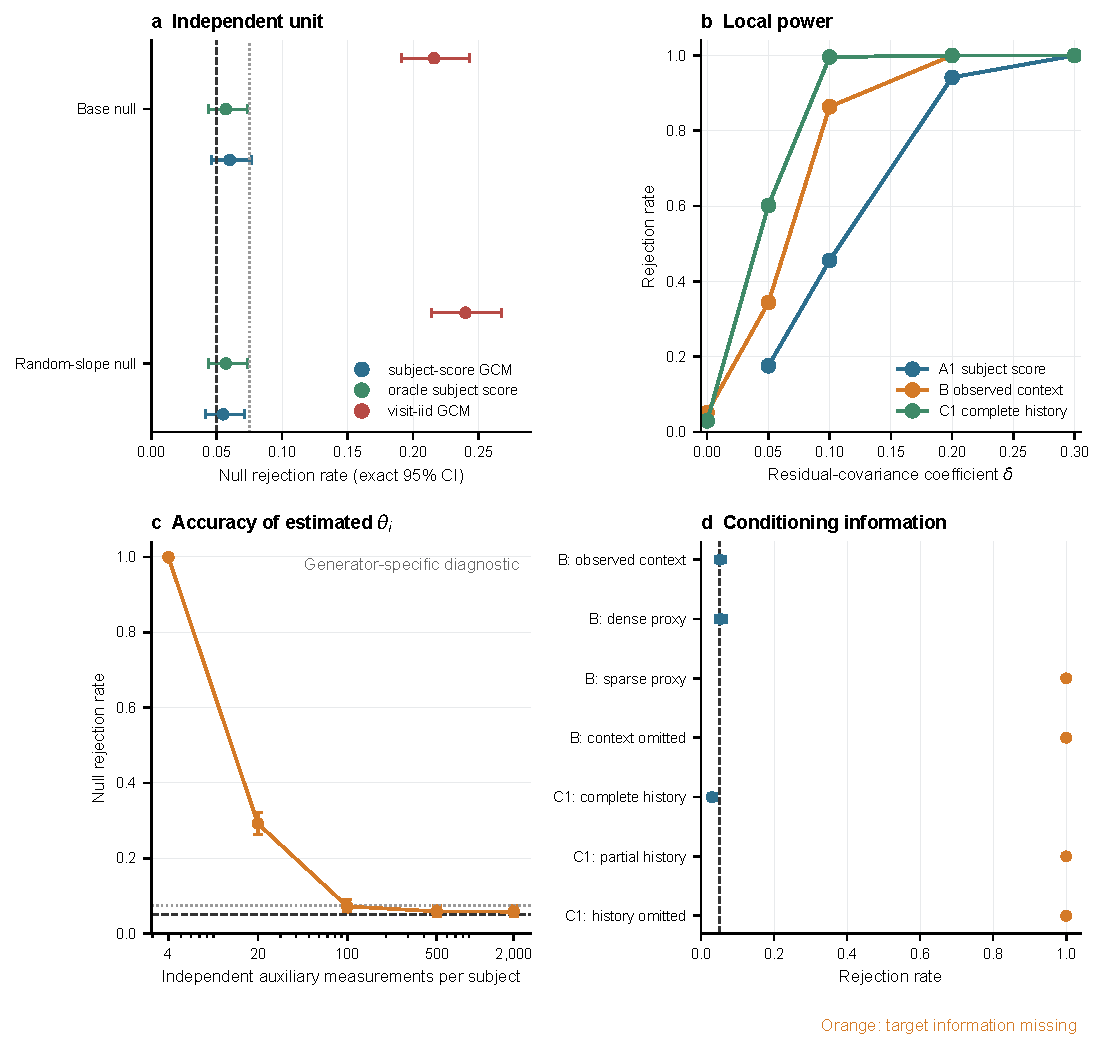
\includegraphics[width=\textwidth]{figure2_simulation_boundaries.pdf}
\caption{Simulation evidence for the framework boundaries. (a) Subject-score and oracle
calculations remain close to the nominal level, while applying the same cross-fitted residual
products as independent visits inflates rejection. The dashed and dotted lines mark 0.05 and
the frozen 0.075 upper-limit criterion. (b) Local power for the A1 subject-score, observed
Case-B, and complete-history C1 constructions; the zero-effect B/C1 points are their frozen
null anchors. (c) Case-B target-null rejection as independently measured subject context
becomes more accurate; this curve is generator-specific. (d) Information-set diagnostics.
Orange rows omit or poorly estimate information in the target conditioning set and therefore
do not estimate Type-I error for the stated target null.}
\label{fig:simulation-boundaries}
\end{figure}

% ============================================================
\section{ADNI applications in the many-subject, sparse-visit regime}

\subsection{Scientific question and data construction}

The Alzheimer's Disease Neuroimaging Initiative (ADNI) is a longitudinal, multisite
observational study \cite{weiner2010}. The first application examined whether a multivariate pattern of
structural brain volumes remained associated with contemporaneous cognitive severity after
adjustment for demographic and technical covariates. MRI atrophy patterns have previously
been associated with ADAS-Cog13 and subsequent cognitive decline in ADNI
\cite{risacher2017}. This MRI analysis used an authorised ADNI Study Files snapshot
downloaded on 26 July 2026. Participant-level source and derived data remain local and are
not redistributed.

Although ADNI is longitudinal, the present asymptotic regime is A1 rather than A2: the
number of participants is large and each participant contributes a small number of irregular
visits. Subject scores, not the length of one time series, drive inference. Time-invariant
observed variables such as APOE genotype enter the conditioning set as observed Case-B
context and remain inside the subject-level fold. No analysis conditions on an estimated
latent subject effect.

Each ADAS13 assessment date served as an anchor. We selected the nearest QC-eligible
FreeSurfer 7 MRI examination within the pre-specified $\pm30$-day window. Ties were broken
by minimum absolute date
gap and then by the earlier MRI date. Before matching, MRI rows had to contain positive,
physiologically plausible required volumes and could not carry an explicit overall,
ventricular, or hippocampal QC failure. Same-day MRI duplicates were resolved by processing
completeness, QC support, field strength, and image identifier without using ADAS13. The
$X$ markers were ventricular volume (bilateral lateral and inferior-lateral ventricles plus
third and fourth ventricles), bilateral hippocampal volume, and bilateral entorhinal volume.
The continuous $Y$ outcome was ADAS13, for which larger values indicate worse cognition.
MRI volumes were measured in mm$^3$.

The conditioning set $Z$ contained time since baseline, baseline age, sex, education, APOE4,
intracranial volume, ADNI protocol, site, MRI field strength, and the MRI--ADAS13 date gap.
Concurrent cognitive scales and diagnosis were excluded: they overlap with ADAS13 or may
represent downstream disease stage rather than baseline confounding. The estimand is the
population-level conditional association between MRI volumes and ADAS13 after adjustment for
these demographic and acquisition variables.

Within 30 days, 8,628 complete matched rows from 2,355 subjects were available. To obtain a
genuinely repeated-measures application and a common cohort in which the
subject-conditional calculation could be evaluated, the analysis cohort required at least
five complete visits. It contained 4,406 observations from 647 subjects; the median was six
visits and the range was five to 13. The median absolute MRI--ADAS13 date gap was one day and
its 90th percentile was 19 days. This visit-enriched cohort targets the repeated-measures
estimand and represents a selected subset of the full ADNI population.

\subsection{Analysis}

Continuous nuisance outcomes were fitted with Gaussian identity-link generalised additive
models. Smooth terms represented time since baseline, baseline age, and intracranial volume;
training fits included a subject random-effect smooth to account for repeated measurements.
Subjects, rather than visits, were assigned to five folds. Held-out predictions excluded the
subject random effect, as required for population-level Design A. Scores used
$w_{it}=1/m_i$, giving every subject equal total weight. The global three-marker test used
9,999 Gaussian multiplier draws; marker-wise $p$-values used a normal reference and Holm
correction.

The date window, minimum visit count, covariates, folds, seed, weights, and inferential rules
were specified before the first GCM analysis. The bounded-visit simulations did not support
Design-B calibration, so real-data inference is restricted to Design A.

\subsection{Results}

The Design A global test rejected the population-level residual-covariance null
($M=13.4028$, empirical multiplier $p=0.0001$). This is the smallest attainable value with
9,999 draws and is not reported as zero. All three marker tests survived Holm correction
(Table~\ref{tab:adni}). Larger residual ventricular volume was associated with higher
ADAS13, while larger residual hippocampal and entorhinal volumes were associated with lower
ADAS13. These directions agree with the medical expectation specified before analysis for
atrophy-related cognitive impairment.

\begin{table}[!ht]
\centering
\caption{MRI--ADAS13 Design A results in 647 ADNI participants. Normalised
covariances divide the raw equal-subject residual covariance by the two corresponding
residual standard deviations. Intervals use the marker-level standard error and a normal
approximation; these quantities are descriptive rather than pre-specified effect sizes.}
\label{tab:adni}
\resizebox{\textwidth}{!}{%
\begin{tabular}{lrrrr}
\toprule
Marker & Normalised covariance & 95\% interval & $T$ & Holm $p$ \\
\midrule
Ventricles & 0.307 & $0.230,\ 0.384$ & 7.850 & $4.16\times10^{-15}$ \\
Hippocampus & $-0.466$ & $-0.536,\ -0.396$ & $-12.979$ & $3.20\times10^{-38}$ \\
Entorhinal & $-0.419$ & $-0.481,\ -0.358$ & $-13.403$ & $1.75\times10^{-40}$ \\
\bottomrule
\end{tabular}
}
\end{table}

Residual means were small relative to their standard deviations: every absolute residual
mean was below 4\% of its corresponding residual standard deviation. The five folds contained
123--136 subjects and 827--924 visits. Removing any single subject preserved every marker
estimate's direction. Maximum absolute standardised subject scores ranged from 6.46 to 7.47,
indicating that influence remains relevant even though no single subject determined a direction.
Complete-case filtering, the at-least-five-visit restriction, ADNI participation, and the
random-slope simulation result define the population to which this analysis most directly applies.

\subsection{What the existing analyses distinguish}

The MRI--ADAS13 analysis also provides a descriptive comparison of association magnitudes;
predictive biomarker performance requires a separate held-out evaluation. After orienting the three anatomical markers
so that larger values represent the adverse direction, the descriptive normalised residual
covariances were 0.307 for ventricles, 0.466 for hippocampus, and 0.419 for entorhinal
cortex. Thus the hippocampal and entorhinal signals were stronger than the ventricular
signal on this residual scale. Because this ordering was examined after the main analysis
and denominator uncertainty was not propagated into formal between-marker comparisons, it
is treated as hypothesis-generating rather than as a ranking of clinical biomarkers.

An earlier cluster-GCM analysis aligned the same three MRI regions to AV45 amyloid PET in
672 observations from 467 participants. It provides a sharper demonstration of the
incremental-information estimand. When concurrent cognition and baseline covariates were in
the reference set, the global test did not reject ($M=1.7663$, $p=0.2124$), and no
marker survived Holm correction (Holm $p=0.8185$, $0.2320$, and $0.8185$ for ventricles,
hippocampus, and entorhinal cortex). In a distinct sensitivity estimand that omitted concurrent
cognition, the global test rejected ($M=6.3355$, empirical $p=0.0001$), and all three
markers survived Holm correction. Their direction-oriented normalised residual covariances
were 0.134, 0.277, and 0.203, respectively. The two results cannot be pooled: they show that
whether MRI is judged to add information depends on what information is already represented
by $Z$.

\begin{table}[!ht]
\centering
\caption{Extent to which the completed ADNI experiments address the core incremental-information
objective. Each conclusion is relative to its named candidate, target, and reference set.}
\label{tab:adni-core-objective}
\small
\begin{tabularx}{\textwidth}{>{\raggedright\arraybackslash}p{0.20\textwidth}
                              >{\raggedright\arraybackslash}X
                              >{\raggedright\arraybackslash}X}
\toprule
Completed analysis & Relation to the core objective & Result and interpretation \\
\midrule
MRI--AV45, cognition-conditioned & Direct test of whether regional MRI ($X$) contains continuous amyloid-PET information ($Y$) beyond cognition and baseline/technical context ($Z$). & Global $p=0.2124$; no marker survived Holm correction. No detectable incremental MRI--amyloid information remained beyond the measured cognitive context. \\
MRI--AV45, baseline-covariate sensitivity & Comparator with cognition removed from $Z$, showing how the answer changes when behavioural context is unavailable. & Global empirical $p=0.0001$; all markers survived Holm correction with coherent directions. MRI carried total residual amyloid signal under this smaller reference set. \\
MRI--ADAS13 & Regional MRI ($X$) and concurrent ADAS13 ($Y$) after demographic and technical adjustment; a supporting application rather than the pathology-beyond-cognition question. & Global empirical $p=0.0001$; all markers survived Holm correction. Supports coherent contemporaneous MRI--cognition signal and method feasibility; pathology-specific and prospective value are addressed by the other designs. \\
Plasma--Centiloid, cognition/genetics-conditioned & Direct test of whether four accessible plasma markers contain amyloid-PET information beyond cognition, demographics, APOE, and acquisition context. & Global empirical $p=0.0001$. Unique-marker tests retained p-tau217 and A$\beta$42/40 but not NfL or GFAP; adding plasma reduced held-out MSE by 29.7\%. The same marker distinction held in 20/20 repeated subject-fold assignments. This is the strongest completed match to the core objective. \\
Plasma--future ADAS13, history-conditioned & Prospective test of whether plasma markers contain prognostic information beyond current cognition, prior cognition, demographics, APOE, and timing. & Global empirical $p=0.0001$. Only p-tau217 retained a unique signal after adjustment for the other markers. Its held-out MSE reduction was 15.2\% in the 30-day cohort and 17.3\% in the 90-day sensitivity cohort; repeated-fold direction and prediction gains were stable, with adjusted detection in 19/20 splits. \\
\bottomrule
\end{tabularx}
\end{table}

The completed MRI--AV45 experiment addresses the core objective for one candidate modality,
one pathology target, and one measured context set. Its primary answer is that no additional
MRI information about amyloid was detected after cognition was included. This separates a
plausible marginal MRI--amyloid signal from incremental information in the analysed cohort.
Concurrent cognition may represent shared disease information, mediation, overadjustment, or
collider distortion, so the reference-set comparison is itself scientifically informative.

The applications support three levels of interpretation. The global test asks
whether the marker panel contributes any residual information. Marker-wise tests identify
which pre-specified measurements contribute detectable residual signal. A stronger claim
that one marker provides unique or practically useful information requires conditioning on
the other markers and demonstrating out-of-subject predictive improvement. The MRI analyses
provide the first two levels; the plasma analyses add unique-marker tests and held-out prediction
on common cohorts (Table~\ref{tab:adni-core-objective}).

\subsection{Plasma information about PET amyloid beyond cognition and genetics}

We next implemented the pre-specified primary pathology-information combination. Amyloid PET
acquisitions were the anchors, with continuous Centiloids as $Y$. The accessible plasma block
$X$ comprised p-tau217, A$\beta$42/40, NfL, and GFAP. The reference set $Z$ comprised concurrent
MOCA, MMSE, and CDR-SB; age, sex, education, APOE $\varepsilon4$ dosage, PET tracer, visit time,
and exact plasma and cognitive date gaps. Plasma and cognition were deterministically matched
within $\pm90$ days. Negative assay missing-value codes were removed before complete-case
construction. The resulting common cohort contained 758 PET-anchored observations from 664
participants; 94 participants had two observations. The median absolute plasma--PET gap was
7 days, its 90th percentile was 42 days, and the maximum was 90 days.

Because most participants contributed one observation, the Design A nuisance models omitted
the computationally redundant subject random-effect smooth, but retained equal-subject training
weights, participant-level folds, participant-level score aggregation, and $\sqrt{N}$ scaling.
This does not change the population-level estimand. The global four-marker test rejected the
conditional residual-covariance null ($M=9.3130$, multiplier $p=0.0001$). On the marker-wise
analysis, p-tau217, A$\beta$42/40, and GFAP survived Holm correction, whereas NfL did not
(Holm $p=0.7557$). Their residual-covariance signs were medically coherent: higher p-tau217
and GFAP and lower A$\beta$42/40 accompanied higher residual Centiloids.

The stronger candidate-discrimination analysis placed the other three plasma markers in the
reference set for each marker in turn. P-tau217 retained a normalised residual covariance of
0.505 (Holm $p=9.19\times10^{-16}$), and A$\beta$42/40 retained $-0.264$
(Holm $p=8.25\times10^{-12}$). By contrast, NfL ($-0.098$, Holm $p=0.1571$) and GFAP
(0.008, Holm $p=0.8559$) did not retain detectable unique amyloid information after the other
plasma markers were included. Thus the result distinguishes an amyloid-focused pair from two
markers whose total signal was shared with that pair. This marker-level separation is
consistent with external evidence
that plasma A$\beta$42/40 and p-tau217 play distinguishable roles in amyloid-related trial
selection and disease monitoring \cite{ashton2022}; that agreement is a biological
plausibility check rather than part of the selection rule (Table~\ref{tab:adni-plasma-amyloid}).

Held-out prediction supplied a separate practical check. Adding the four plasma markers to the
same reference model reduced participant-level standardised-outcome RMSE from 0.794 to 0.666,
equivalent to a 29.7\% mean-squared-error reduction. A participant bootstrap gave a positive
mean MSE improvement interval of 0.126--0.250 and one-sided $p=0.0001$. The global test,
unique-marker pattern, and held-out gain therefore agree that plasma is the completed ADNI
combination that best instantiates the paper's core objective.

Twenty additional subject-fold assignments held the cohort, variables, and formulas fixed.
P-tau217 remained positive and Holm-significant in 20/20 assignments, with normalised
covariances from 0.456 to 0.497; A$\beta$42/40 remained negative and significant in 20/20,
from $-0.276$ to $-0.244$. NfL and GFAP were detected in 0/20 assignments. The plasma-block
MSE reduction was positive in every assignment, with a median of 27.9\% and a range of
25.4\%--29.3\%. These repeated folds quantify algorithmic stability within the selected cohort.

A direct cross-modality check used the 570 participants (641 observations) with both plasma
and a QC-eligible structural MRI within 90 days of PET. After moving the MRI block into $Z$,
the plasma block remained detectable (global $p=0.0001$); after moving the plasma block into
$Z$, the MRI block did not ($p=0.2378$). On the same folds and cohort, plasma reduced held-out
MSE by 28.8\%, MRI by 0.3\%, and both together by 29.2\%. This common-cohort result, rather
than unequal-sample $p$-value ranking, is the basis for selecting plasma--Centiloid as the
current primary real-data experiment.
Figure~\ref{fig:adni-signature} places this common-cohort comparison next to the unique-marker
and prospective results.

\begin{table}[!ht]
\centering
\caption{Unique-marker plasma--amyloid results after conditioning on cognition,
genetics, acquisition context, and the other three plasma markers.}
\label{tab:adni-plasma-amyloid}
\begin{tabular}{lrrl}
\toprule
Marker & Normalised covariance & Holm $p$ & Incremental-information conclusion \\
\midrule
p-tau217 & 0.505 & $9.19\times10^{-16}$ & detected \\
A$\beta$42/40 & $-0.264$ & $8.25\times10^{-12}$ & detected \\
NfL & $-0.098$ & 0.1571 & not detected \\
GFAP & 0.008 & 0.8559 & not detected \\
\bottomrule
\end{tabular}
\end{table}

\subsection{Prospective plasma information about future cognition given observed history}

We next used the bounded observed-history branch C1 to address prognosis. Plasma assay dates
served as candidate index dates. The marker block $X$ contained log-transformed p-tau217,
A$\beta$42/40, NfL, and GFAP. The outcome $Y$ was a future ADAS-Cog13 assessment between 270
and 1,278 days after the index. When several assessments were available, we selected the one
closest to 730 days. The reference set $Z$ contained age, sex, education, APOE $\varepsilon4$
dosage, concurrent ADAS-Cog13, and the current and future date gaps. The observed history
$H_{it}$ contained the most recent ADAS-Cog13 score from 180--1,080 days before the index and
its date gap. APOE was observed stable Case-B context rather than an estimated latent effect.

We retained the earliest eligible index date for each participant. The primary $\pm30$-day
current-assessment window produced 199 independent participant rows. The median absolute
current gap was zero days. The median prior-assessment gap was 384 days, and the median
future-assessment gap was 526 days. The future-gap interquartile range was 373--740 days. A
pre-specified $\pm90$-day sensitivity window produced 203 participants. Subject-level
five-fold cross-fitting was retained, although each selected participant contributed one
index row.

The primary four-marker maximum test rejected the history-conditioned residual-covariance
null ($M=4.2330$, multiplier $p=0.0001$). Each unique-marker test also conditioned on the
other three plasma measurements. P-tau217 retained a normalised residual covariance of 0.321
(Holm $p=0.00123$). A$\beta$42/40, NfL, and GFAP did not retain detectable unique information
(Table~\ref{tab:adni-prospective}). Deleting any one participant left the p-tau217 unique-marker
$p$-value between $8.01\times10^{-5}$ and $5.59\times10^{-4}$. The $\pm90$-day sensitivity
analysis gave the same marker distinction, with a p-tau217 normalised covariance of 0.285 and
Holm $p=0.000380$. Independent multicohort work has likewise found that plasma p-tau217 is
associated with future cognitive decline and can complement tau PET \cite{ossenkoppele2025}.
The present analysis isolates its incremental information in the specified ADNI cohort and
conditioning set.

Across 20 additional subject-fold assignments in the primary cohort, the p-tau217 unique
covariance remained positive, with a median of 0.297 and a range of 0.230--0.351. A
conservative four-marker Bonferroni adjustment remained below 0.05 in 19/20 assignments; the
largest adjusted value was 0.098. The direction is therefore stable, while the binary
significance decision shows mild split sensitivity in this smaller cohort.

\begin{table}[!ht]
\centering
\caption{Prospective unique-marker results for future ADAS-Cog13. Every test conditions on
current cognition, prior cognition, demographics, APOE, timing, and the other plasma markers.}
\label{tab:adni-prospective}
\begin{tabular}{lrrrl}
\toprule
Marker & Primary covariance & Primary Holm $p$ & 90-day Holm $p$ & Unique information \\
\midrule
p-tau217 & 0.321 & 0.00123 & 0.000380 & detected \\
A$\beta$42/40 & 0.096 & 0.3988 & 0.2078 & not detected \\
NfL & 0.057 & 0.7362 & 0.7131 & not detected \\
GFAP & $-0.054$ & 0.7362 & 0.8215 & not detected \\
\bottomrule
\end{tabular}
\end{table}

Held-out prediction provided a complementary practical comparison. Adding p-tau217 to the
history-conditioned reference reduced RMSE from 5.851 to 5.387, a 15.2\% MSE reduction. The
participant bootstrap interval for the mean MSE reduction was $-0.496$ to 11.006, with a
one-sided $p=0.0375$. The interval crosses zero, so the primary prediction gain is suggestive
under a two-sided 95\% criterion. In the 90-day sensitivity cohort, RMSE fell from 5.886 to
5.351. The corresponding 17.3\% MSE reduction had a bootstrap interval of 0.334--12.231 and
one-sided $p=0.0186$. By contrast, adding prior cognition to the current-cognition reference
reduced MSE by only 1.9\% in the primary cohort. The history remains part of the conditioning
set because it defines the scientific null, not because it must improve prediction strongly.
Across the 20 repeated fold assignments, the p-tau217 MSE reduction was positive every time,
with a median of 21.0\% and a range of 14.6\%--26.6\%.

This prospective result distinguishes candidate markers instead of reporting only association
directions. P-tau217 was the only marker supported by the unique-information test, the
leave-one-participant-out check, and held-out prediction. The analysis belongs to the
many-subject C1 branch, which reduces to A1 after adding fixed observed history; the
single-series temporal theory discussed by Shi instead motivates the growing-history C2 branch.

\subsection{Additional ADNI conditional pathology-information targets}

The completed plasma--amyloid experiment retains the scientific structure of the original IWSM example:
does an accessible candidate measurement $X$ contain information about established disease
pathology $Y$ beyond clinical or behavioural context $Z$? The remaining MRI block contains
hippocampal, entorhinal, and ventricular measures. A second pathology target is
temporal-meta-ROI tau PET SUVR, for which amyloid burden is added to $Z$ so that the target
is tau information beyond amyloid stage. The reference set also contains contemporaneous
cognition, age, sex, education, site/phase, visit time, assay and imaging versions, and exact
date gaps. APOE $\varepsilon4$ dosage and a frozen externally weighted non-APOE polygenic
score form a time-invariant genetic background block $G_i$. They enter $Z$ for plasma and
MRI tests. In a reciprocal analysis, $G_i$ is instead the candidate $X$ and is not repeated
as though each visit supplied a new genotype observation.

PET acquisition dates anchor the primary alignment. Plasma, MRI, and cognition are matched
using continuous dates inside a frozen $\pm90$-day window; $\pm180$ days is a sensitivity
analysis. All visits for one participant remain in one fold, and repeated residual products
are aggregated to one equal-subject score. The APOE-adjusted cohort is analysed without
requiring a non-APOE score for everyone; the polygenic extension has its own documented
complete-case cohort.

Candidate discrimination was pre-specified at five levels:
\begin{enumerate}[leftmargin=*]
\item a global test across all frozen candidates;
\item multiplicity-adjusted plasma, MRI, and genetic block tests;
\item unique-block tests that move the other candidate blocks into $Z$;
\item Holm-adjusted marker-wise and within-block unique-marker tests; and
\item participant-held-out changes in RMSE and MAE for continuous PET, with AUC and Brier-score
changes for a secondary frozen PET-positivity threshold.
\end{enumerate}
Candidate ranking is based on a common comparison cohort, cross-fitted scale-normalised residual covariances,
participant-bootstrap intervals for their pairwise differences, unique-information tests,
and paired prediction-loss changes. Maximal cohorts for individual blocks are sensitivity
analyses rather than a basis for ranking unequal-sample p-values.

The completed amyloid result supplies the first candidate-by-target information signature rather than a
list of signs: p-tau217 and A$\beta$42/40 retained unique amyloid information, whereas NfL and
GFAP did not. For the remaining target, plasma p-tau217 is expected to carry tau information;
NfL and structural MRI should be more closely
related to neurodegeneration and subsequent cognition; and genetic risk may attenuate once
measured pathology enters $Z$ \cite{janelidze2024,moon2025}. These frozen qualitative
expectations serve as external plausibility checks while leaving discordant results reportable. An ADNI4 remote extension can treat
Storyteller speech features or ECog-12 as accessible $X$, standard cognitive measures and
genetics as $Z$, and blood or PET pathology as $Y$. It is promoted only if continuous-date
linkage and pathology overlap are adequate \cite{skirrow2024}.

Together, the prospective cognitive target and the pathology-information target preserve the
link between the IWSM example and future wearable applications. Tau PET and a frozen non-APOE
polygenic score are the next conditional pathology-information targets.

\begin{figure}[!ht]
\centering
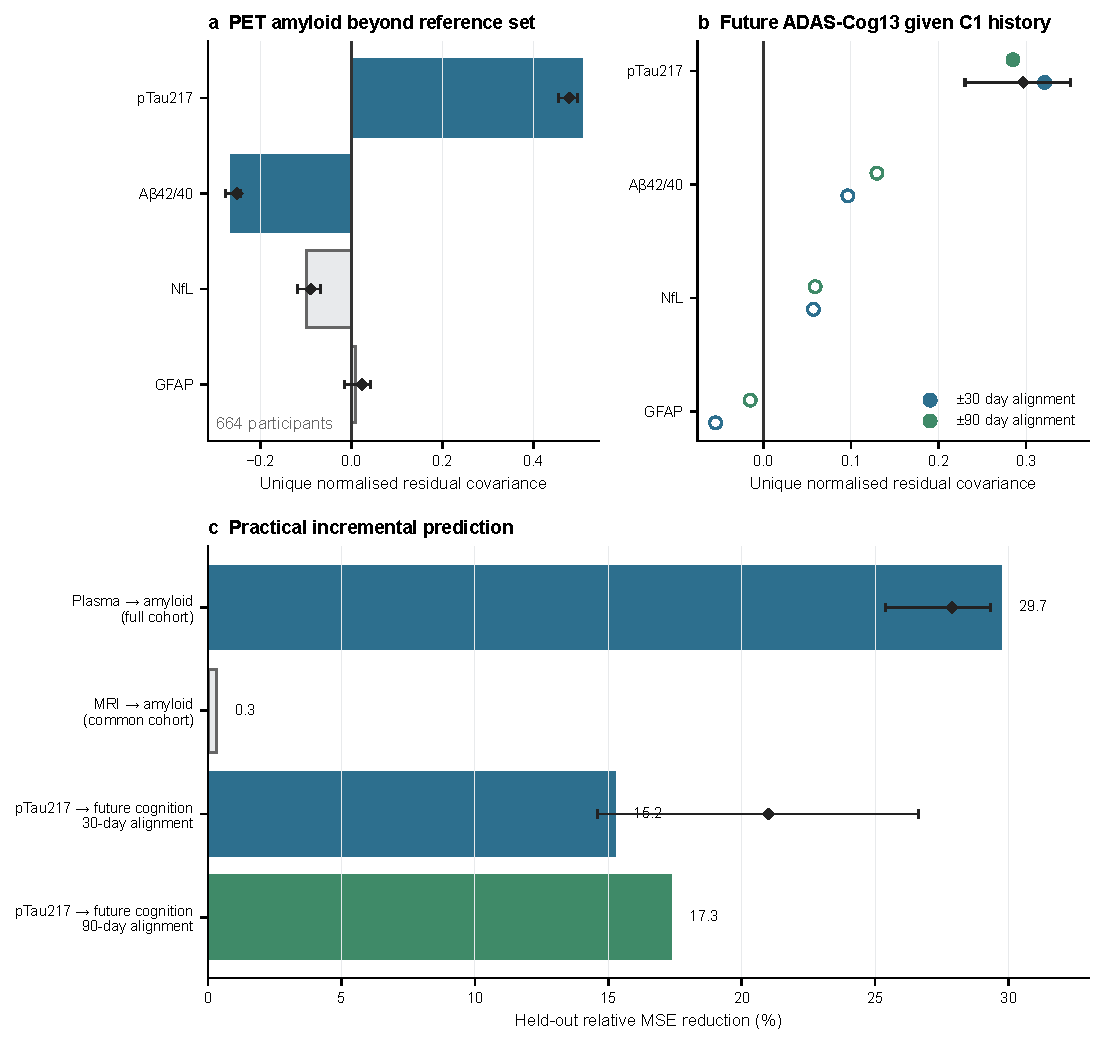
\includegraphics[width=\textwidth]{figure3_adni_information_signature.pdf}
\caption{ADNI candidate-information signatures rather than sign recovery alone. (a) Unique
plasma-marker residual covariances with PET amyloid after conditioning on cognition,
demographics, APOE, acquisition context, and the other plasma markers; blue bars survive
Holm correction. Black diamonds and whiskers show the median and range across 20 additional
subject-fold assignments. (b) Unique plasma information about future ADAS-Cog13 after current and
prior cognition (C1); filled points survive Holm correction. (c) Participant-held-out
prediction gains. Plasma added substantially more predictive information than structural
MRI, and p-tau217 improved future-cognition prediction under both alignment windows.
Repeated-fold diamonds and whiskers are shown for the full plasma cohort and primary
future-cognition analysis.}
\label{fig:adni-signature}
\end{figure}

% ============================================================
\section{Discussion}

The central contribution is a separation principle: the target null, the available
conditioning information, and the independent asymptotic unit must be chosen before the
nuisance learner. The five cases make this principle operational. A1 uses independent
subject scores; A2 and C2 derive information from time; A3 needs two-rate asymptotics; B can
contain a generated-variable or latent-variable identification problem; C1 can reduce to A1;
and D/E concern stochastic paths. Calling all of these settings ``mixed GCM'' would obscure
the change in target and reference distribution.

Within A1, subject aggregation aligns the score, variance estimate, and cross-fitting unit.
The direct method comparison makes the consequence visible: using the same cross-fitted
residuals but treating visits as independent produced null rejection rates above 0.20,
whereas subject scores closely tracked the oracle. The wider simulation programme also
defines the current boundary. The core null and five of six Stage-2b settings met the frozen
criterion, while the original random-slope stress setting did not. Observed Case-B context
and complete C1 history calibrated well; a dense auxiliary proxy succeeded in its favourable
generator, but a sparse proxy and incomplete history did not recover the target null. The
new proxy gradient sharpens that statement: calibration improved continuously with auxiliary
accuracy, and even 500 measurements narrowly missed the strict frozen gate in this generator.
The local-power curves show useful sensitivity before the ceiling effects of the original
strong alternatives.

The ADNI analyses show why the conditioning set is scientifically consequential. Structural
MRI retained coherent contemporaneous information about ADAS-Cog13, but did not retain
detectable amyloid-PET information once concurrent cognition entered the reference set. In
the primary pathology experiment, p-tau217 and A$\beta$42/40 retained unique information
about Centiloid, while NfL and GFAP did not. On a common cohort, plasma reduced held-out MSE
by 28.8\%, compared with 0.3\% for structural MRI. In the prospective C1 analysis, p-tau217
was the only plasma marker with unique information about future ADAS-Cog13 and reduced
held-out MSE by 15.2\%--17.3\%. Repeated subject folds preserved the plasma--amyloid
two-marker distinction and positive prediction gain in every assignment. The prospective
p-tau217 direction and prediction gain were also stable, although one of 20 assignments did
not cross the adjusted 0.05 threshold. The contribution is therefore a candidate-information
signature relative to a named reference set, rather than recovery of plausible signs alone.

GTCM and DNCIT identify two natural extensions. GTCM supplies a route to temporally
dependent residual scores for growing-history C2; DNCIT supplies conditions for composing a
learned representation of high-dimensional $X$ with a downstream CIT. A future hybrid must
satisfy both representation-training and non-i.i.d. calibration conditions. The motivating
private wearable application has the same scientific form---whether device signals contain
outcome information beyond recorded activity---but no private wearable data or result enters
this article.

Three limitations remain central. The A1 result is currently a high-level theorem and proof
roadmap rather than a submission-complete technical proof. The scalar residual covariance is
not omnibus against conditional-dependence alternatives with zero conditional covariance.
Finally, the ADNI findings are observational, complete-case, and exploratory; they establish
neither causality nor clinical biomarker qualification. These limits determine the next
theoretical and empirical steps rather than changing the five-case taxonomy.

% ============================================================
\section{Reproducibility, data availability, and governance}

The analysis code, pre-specified settings, separately stored Monte Carlo repetitions,
summary tables, and dated validation reports are organised in the accompanying EGCM
repository \cite{huo2026} and at \url{https://github.com/Aokowww/EGCM}. The MRI--ADAS13
Design A analysis recorded SHA-256 hashes for the
analysis table, settings, complete results, and summary tables. The analytic input
contained 4,406 rows from 647 subjects; its SHA-256 hash begins
\texttt{bb426c9b0df2}, with the complete value retained in the dated experiment record.
ADNI source and participant-level derived files are excluded from version control and cannot
be redistributed. Reproduction of the application requires separately approved ADNI access
and the documented source-table versions. The plasma--amyloid analysis used the 12 August
2026 UPENN plasma and UC Berkeley amyloid-PET Study Files snapshots. Restricted rows were
processed locally; only aggregate, disclosure-checked cohort, test, unique-marker, and
prediction summaries are retained in the public repository. Its analytic table contained
758 rows from 664 participants; the SHA-256 begins \texttt{d218c64b6c0d}. Remaining analyses
must follow the same restricted-data boundary. The prospective analysis used a local
ADNIMERGE2 archive obtained on 23 August 2026 and wrote no participant-level derived table.
Its code and frozen configuration hashes begin \texttt{5ff00256d72b} and
\texttt{e8d930856e5e}. Public cohort, marker, and prediction files contain aggregate rows only.
The repeated-fold ADNI extensions retained only split-level aggregate statistics. For the
plasma--amyloid analysis, the configuration, runner, and public summary hashes begin
\texttt{1327be144ff8}, \texttt{68b842d657e4}, and \texttt{0c00c0e32d6d}. For prospective
C1, the corresponding hashes begin \texttt{70bca1df4fc2}, \texttt{b4e2be9b7035}, and
\texttt{28c5917892c5}. No fold membership, residual, row-level prediction, identifier, or date
is released.

The Case-B/C extension was frozen before its 1,000-repetition run. Its configuration,
simulation script, dated plan, aggregate summary, replicate-level results, and validation
report are retained separately. The SHA-256 hashes of the configuration and aggregate
summary begin \texttt{aee6ba192f65} and \texttt{beb66ef1df74}, respectively. The experiment
contains synthetic data only. No wearable-study row or other private application data were
used.

The supplementary B/C1 gradient comprised 9,000 synthetic data sets. The SHA-256 hashes of
its configuration, runner, aggregate summary, and replicate-level results begin
\texttt{0e8d54662bcf}, \texttt{cb83c321b8e7}, \texttt{7219a60e54cf}, and
\texttt{fc134d143ad0}. Only the aggregate summary is included in the public artifact.

The inferential-unit comparison was frozen before its 4,000 simulated data sets were run.
The SHA-256 hashes of its configuration, simulation script, and full aggregate summary begin
\texttt{69a947f1cc25}, \texttt{1ce8fa18bbd2}, and \texttt{218e3c4b6098}, respectively.
Replicate-level results remain outside the public release; the disclosure-safe aggregate
summary and validation record are public.

ADNI source data are available to approved investigators through the Image and Data Archive,
subject to the ADNI Data Use Agreement and publication policy. The present work is a
secondary analysis of de-identified data and involved no new participant contact or data
collection. ADNI study protocols were approved by the participating sites and written
informed consent was obtained under those protocols \cite{weiner2010}.

% ============================================================
\section{Limitations and next directions}

The first priority is a submission-complete proof of the A1 result, including the oracle
cluster central limit theorem, cross-fitted remainder bounds, score-variance consistency,
and fixed and local alternatives. Any response to the original Stage-2b random-slope failure
must be evaluated under a newly frozen method version rather than tuned against that row.

A2 and A3 require separate theory. A2 needs a temporal score process, weak-dependence or
martingale conditions, and long-run variance or self-normalised calibration. A3 must state
joint growth conditions for $N$, $T_i$, and the largest cluster contribution. In Case B,
sufficient rates are needed when $\widehat\theta_i$ is estimated from independent auxiliary
data, together with additional leakage terms when it is learned from the same trajectory.
Sparse BLUPs remain a negative control unless a model-specific identification theorem is
available.

For C2, future simulations should vary history length, mixing strength, proxy accuracy, and
local alternative size, followed by a growing-history theorem comparable in purpose to the
GTCM stability argument. Learner-specific corollaries for GAMMs, kernel ridge regression,
and other regressions can be stated through common prediction-rate conditions. A
high-dimensional extension must additionally combine DNCIT-style representation separation
with subject-level splitting and non-i.i.d. calibration.

Cases D and E require a path-space estimand and a trajectory-level score before calibration
can be addressed. Empirically, tau-PET, genetic, and independent ADNI snapshot analyses
should be frozen separately from the completed same-time and future-cognition experiments.
Repeated folds quantify algorithmic sensitivity but do not replace temporal or external-
cohort validation. Only aggregate, disclosure-checked outputs may enter public artifacts.

% ============================================================
\section{Scope and evidence summary}

\begin{center}
\small
\setlength{\tabcolsep}{4pt}
\begin{tabular}{>{\raggedright\arraybackslash}p{0.09\textwidth}
                >{\raggedright\arraybackslash}p{0.22\textwidth}
                >{\raggedright\arraybackslash}p{0.22\textwidth}
                >{\raggedright\arraybackslash}p{0.20\textwidth}
                >{\raggedright\arraybackslash}p{0.17\textwidth}}
\toprule
Case & Scientific target & Theoretical status & Empirical evidence & Interpretation \\
\midrule
A1 & state-level, many subjects & developed proof programme under cluster rates & Stage 2a; six stress settings; ADNI & primary current scope \\
A2 & state/predictive, long sequence & requires temporal theory & Shi/GTCM comparison only & not implemented here \\
A3 & state-level, both dimensions grow & requires double asymptotics & none & future theory \\
B & state-level given $\theta_i$ & observed case reduces to A; latent case conditional & observed context, proxy-quality gradient, and local power & heuristic if estimated \\
C1/C2 & state-level given history & bounded-history C1 reduces to A1; growing-history C2 is temporal & C1 calibration/local power plus prospective ADNI and repeated folds & regime-dependent \\
D/E & trajectory-level paths & no theorem here & none & future work \\
\bottomrule
\end{tabular}
\end{center}

% ============================================================
\section*{Acknowledgements}

Data used in preparation of this article were obtained from the Alzheimer's Disease
Neuroimaging Initiative (ADNI) database. As such, the investigators within ADNI contributed
to the design and implementation of ADNI and/or provided data but did not participate in the
analysis or writing of this report. A complete listing of ADNI investigators can be found at
\url{https://adni.loni.usc.edu/wp-content/uploads/how_to_apply/ADNI_Acknowledgement_List.pdf}.

Data collection and sharing for ADNI are funded by the National Institute on Aging (National
Institutes of Health Grant U19AG024904). The grantee organisation is the Northern California
Institute for Research and Education. In the past, ADNI also received funding from the
National Institute of Biomedical Imaging and Bioengineering, the Canadian Institutes of
Health Research, and private-sector contributions through the Foundation for the National
Institutes of Health, including AbbVie; Alzheimer's Association; Alzheimer's Drug Discovery
Foundation; Araclon Biotech; BioClinica, Inc.; Biogen; Bristol-Myers Squibb Company;
CereSpir, Inc.; Cogstate; Eisai Inc.; Elan Pharmaceuticals, Inc.; Eli Lilly and Company;
EuroImmun; F. Hoffmann-La Roche Ltd and its affiliated company Genentech, Inc.; Fujirebio;
GE Healthcare; IXICO Ltd.; Janssen Alzheimer Immunotherapy Research \& Development, LLC;
Johnson \& Johnson Pharmaceutical Research \& Development LLC; Lumosity; Lundbeck; Merck
\& Co., Inc.; Meso Scale Diagnostics, LLC; NeuroRx Research; Neurotrack Technologies;
Novartis Pharmaceuticals Corporation; Pfizer Inc.; Piramal Imaging; Servier; Takeda
Pharmaceutical Company; and Transition Therapeutics.

\begin{thebibliography}{99}

\bibitem{shahpeters}
R. D. Shah and J. Peters.
\newblock The hardness of conditional independence testing and the generalised covariance measure.
\newblock \emph{The Annals of Statistics}, 48(3):1514--1538, 2020.

\bibitem{fukumizu2007}
K. Fukumizu, A. Gretton, X. Sun, and B. Sch\"olkopf.
\newblock Kernel measures of conditional dependence.
\newblock In \emph{Advances in Neural Information Processing Systems 20}, pages 489--496, 2007.

\bibitem{zhang2011}
K. Zhang, J. Peters, D. Janzing, and B. Sch\"olkopf.
\newblock Kernel-based conditional independence test and application in causal discovery.
\newblock In \emph{Proceedings of the 27th Conference on Uncertainty in Artificial Intelligence},
pages 804--813, 2011.

\bibitem{scheidegger2022}
C. Scheidegger, J. H\"orrmann, and P. B\"uhlmann.
\newblock The weighted generalised covariance measure.
\newblock \emph{Journal of Machine Learning Research}, 23(273):1--68, 2022.

\bibitem{bellot2019}
A. Bellot and M. van der Schaar.
\newblock Conditional independence testing using generative adversarial networks.
\newblock In \emph{Advances in Neural Information Processing Systems 32}, 2019.

\bibitem{chwialkowski2014}
K. Chwialkowski and A. Gretton.
\newblock A kernel independence test for random processes.
\newblock In \emph{Proceedings of the 31st International Conference on Machine Learning},
volume 32 of \emph{Proceedings of Machine Learning Research}, pages 1422--1430, 2014.

\bibitem{huo2026}
Q. Huo, M. Simnacher, X. Xu, and S. Greven.
\newblock Extending the generalised covariance measure for conditional independence testing in repeated-measures data.
\newblock In \emph{Proceedings of the 40th International Workshop on Statistical Modelling}, 2026.

\bibitem{shi2025}
J. Shi.
\newblock Conditional independence testing in time series: a primer.
\newblock Statistical Science Seminar, University College London, 5 February 2025.

\bibitem{wiecksosa2025}
M. Wieck-Sosa, M. F. C. Haddad, and A. Ramdas.
\newblock Conditional independence testing with a single realization of a multivariate
nonstationary nonlinear time series.
\newblock \emph{arXiv preprint arXiv:2504.21647}, 2025.

\bibitem{simnacher2024}
M. Simnacher, X. Xu, H. Park, C. Lippert, and S. Greven.
\newblock Deep nonparametric conditional independence tests for images.
\newblock \emph{arXiv preprint arXiv:2411.06140}, 2024.

\bibitem{wood2017}
S. N. Wood.
\newblock \emph{Generalized Additive Models: An Introduction with R}.
\newblock Chapman and Hall/CRC, second edition, 2017.

\bibitem{weiner2010}
M. W. Weiner et al.
\newblock The Alzheimer's Disease Neuroimaging Initiative: progress report and future plans.
\newblock \emph{Alzheimer's \& Dementia}, 6(3):202--211.e7, 2010.

\bibitem{risacher2017}
S. L. Risacher, W. H. Anderson, A. Charil, P. F. Castelluccio, S. Shcherbinin,
A. J. Saykin, A. J. Schwarz, and the Alzheimer's Disease Neuroimaging Initiative.
\newblock Alzheimer disease brain atrophy subtypes are associated with cognition and rate of decline.
\newblock \emph{Neurology}, 89(21):2176--2186, 2017.

\bibitem{janelidze2024}
S. Janelidze et al.
\newblock Plasma phosphorylated tau 217 and A$\beta$42/40 to predict early brain
A$\beta$ accumulation in people without cognitive impairment.
\newblock \emph{JAMA Neurology}, 81(9):947--958, 2024.

\bibitem{ashton2022}
N. J. Ashton et al.
\newblock Differential roles of A$\beta$42/40, p-tau231 and p-tau217 for Alzheimer's trial
selection and disease monitoring.
\newblock \emph{Nature Medicine}, 28:2555--2562, 2022.

\bibitem{ossenkoppele2025}
R. Ossenkoppele et al.
\newblock Plasma p-tau217 and tau-PET predict future cognitive decline among cognitively
unimpaired individuals: implications for clinical trials.
\newblock \emph{Nature Aging}, 5:883--896, 2025.

\bibitem{moon2025}
H. Moon, X. Chen, and the Alzheimer's Disease Neuroimaging Initiative.
\newblock Plasma p-tau217 predicting brain-wide tau accumulation in preclinical AD.
\newblock \emph{The Journal of Prevention of Alzheimer's Disease}, 12(7):100252, 2025.

\bibitem{skirrow2024}
C. Skirrow et al.
\newblock Storyteller in ADNI4: application of an early Alzheimer's disease screening tool
using brief, remote, and speech-based testing.
\newblock \emph{Alzheimer's \& Dementia}, 20(10):7273--7290, 2024.

\end{thebibliography}

\end{document}
